\begin{savequote}[75mm]
Optical Illusion is optical truth! ... In them is evidenced the living interaction of our inner nature with outer nature.
\qauthor{Johann Wolfgang von Goethe}
\end{savequote}

%For an example of a full page figure, see Fig.~\ref{fig:myFullPageFigure}.
\chapter{Model-Based Point Cloud Tracking}
\label{Chap:ModelBasedTracking}
\lettrine[lines=3, loversize=0.3]{\textcolor{Silver}N}{ow that we have established} a reduced, stable world model in which voxels persist through occlusions, the next step is to adapt the general framework of \gls{sbf} to track models within this 3D voxel world. For an introduction to the general framework of \gls{sbf}, we refer the reader to Appendix \ref{chap:SeqBayesEst}). In this Chapter we begin by presenting the basic framework of particle filter tracking in 3D point clouds, and show how point correspondences can be used to evaluate the particle filtering likelihood function.

While the correspondence approach is feasible for tracking single targets, it suffers from the same flaw as other approaches when extended to multiple targets \cite{MCMCPartFilt_05, ApproxMultiTrack_06,Koo_IROS2013, Breitenstein_ICCV2009} - it significantly increases the computational resources required. This increase is due to the need for more particles - due to assignment of particles to individual targets, a larger state space, or independent filters for each target. While there has been work addressing this problem by offloading processing to a GPU \cite{Choi_IROS2013}, in this work we take a different approach, and search for fundamental changes to the point cloud correspondence particle filter which can reduce computational complexity without affecting accuracy. 

This Chapter is organized as follows: First, in Section \ref{sec:PartFilt3d} we present a framework for particle filter tracking in point clouds using point correspondences. In Section \ref{sec:StratCorrSampling} we present the primary contribution of this Chapter; the use of a supervoxel-based stratified sampling approach to greatly reduce the computational complexity of point cloud correspondence particle filtering. Finally, in Section \ref{sec:ExperimentalResults} we will show that the approach allows performance (on a standard CPU) exceeding that which can be obtained on a recent GPU implementation \cite{Choi_IROS2013}. Furthermore, we shall present extensive quantitative experiments demonstrating the benefits of this approach, as well as show qualitative results from a real-world application. 

\section{Particle Filters in 3D}
\label{sec:PartFilt3d}
The underlying mechanics of 3D point cloud correspondence particle filtering remain the same as in Chapter \ref{Chap:VideoSegRelaxation}, and so we shall not discuss them extensively here; for a detailed introduction to the topic, we again refer the reader to \cite{Doucet2001} or \cite{SequentialMonteCarloMultitargetFiltering}. Rather, we shall only discuss the aspects that differentiate it - the models and how they are scored and propagated. The models here consist of point clouds, and the measurement function relies on point to point correspondence for scoring, rather than a global per-detection metric (such as a histogram distance, used in the 2D trackers of in Chapter \ref{Chap:VideoSegRelaxation}). The dynamic model uses real-world 3D coordinates which also include orientation, rather than 2D pixel coordinates in the image plane. The primary novelty of the approach we present here lies in how we score individual particle predictions using the measurement model. 

\subsection{Model Representation}
One of the main limitations of the 2D projected mask model discussed in Chapter \ref{Chap:VideoSegRelaxation} is that the masks of objects are not invariant to pose changes - in general, rotation of an object will change the shape of its mask and distribution of its color histogram. As we now have the ability to observe the full 3D shape of an object, we choose to represent objects as clusters of points which correspond to the exterior of the object. A visual representation of such a model is given in Figure \ref{fig:ModelExample}.

\begin{figure*}[!ht]
  \centering
  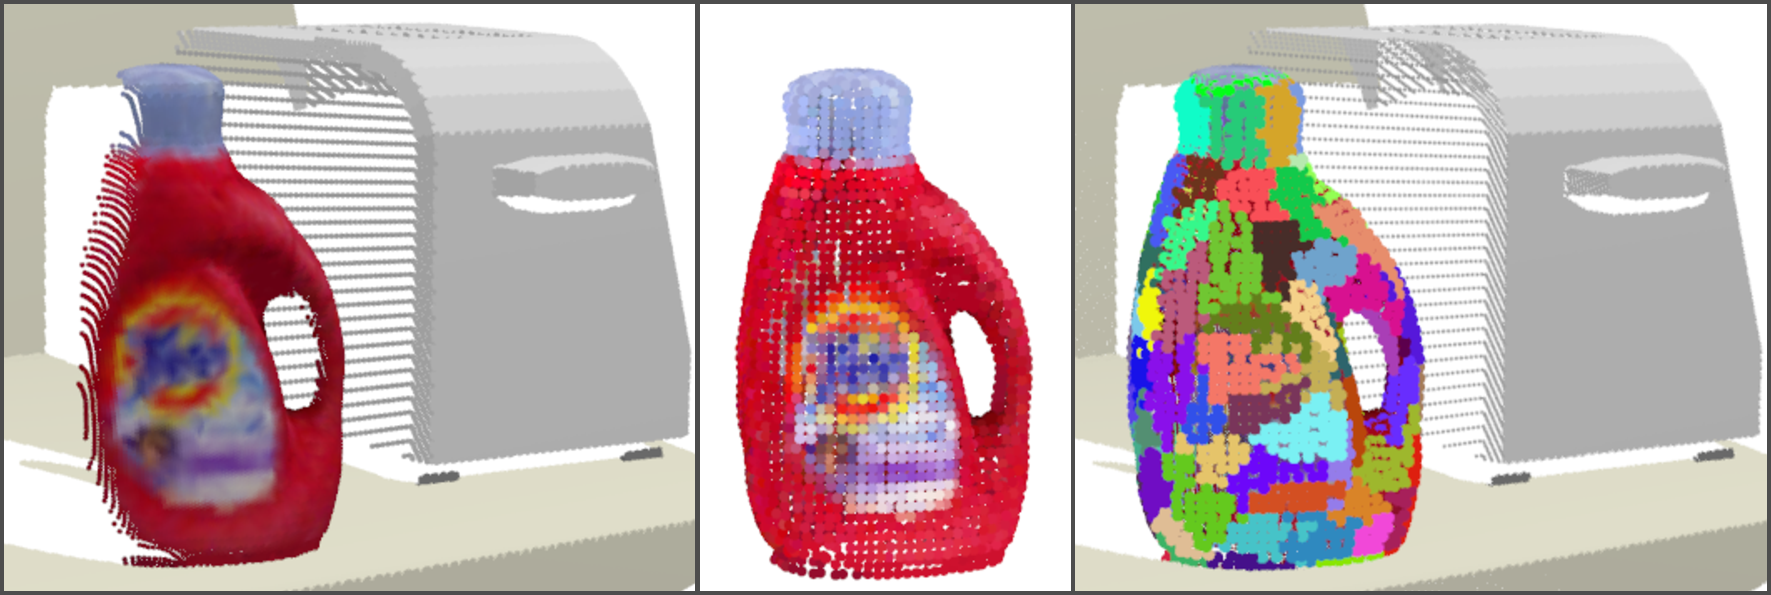
\includegraphics[width=1.0\textwidth]{figures/Tracking/TideModelSV.pdf}
  \caption[Example of data from ``Tide'' sequence.]{Example of data from ``Tide'' sequence. The left frame shows an example of the raw input cloud. Sampling effects from the synthetic RGB-D camera are visible in the quantization of points, especially on the edges of objects. The middle frame shows the voxelized model representation we use, while the right frame shows an example of supervoxel strata used for sampling with $R_{seed} = 0.07m$.}
  \label{fig:ModelExample}
\end{figure*}

Points for objects are stored in a model-centered reference frame (which we shall denote with superscript $^m$), with each point containing an XYZ position, an RGB color for the point, as well as a surface normal vector. That is, each point $p$ of the model $k$ consists of a nine-dimensional vector: 

\begin{equation} \label{eqn:point}
p^m_k = [x^m,y^m,z^m,R,G,B,n_x,n_y,n_z],
\end{equation}
 
 and a model for an object $O_k$ consists of a vector of $n_k$ such points $p^m$:
 
 \begin{equation} \label{eqn:model}
 O^m_k = [p^m_0 ... p^m_{n_k}].
\end{equation}

It is important to note that the points of an object model given above are model-relative - they must be transformed into the world coordinates in order to evaluate their fit to observations. This will be discussed further in the next Section.


\subsection{Dynamic Model}
\label{sec:Dynamic_model}
In the 2D tracker presented previously, the time-dependent state vector of a particle consisted of a position shift vector $\mathbf{p}_t=[p_x,p_y]$ and a velocity vector $\mathbf{v}_t=[v_x,v_y]$. The natural extension of this to 3D is to simply add a third $p_z$ and $v_z$ element to each. Of course we should note that the $x$ and$y$ dimensions here in our 3D representation are distinct from those in 2D, which represented pixel coordinates in the image plane. Here our positional coordinates represent real-world distances from a fixed origin (typically the camera ``pin-hole'' position). It is also important to note that coordinates in our 3D representation are originally in a continuous space - though we discretize them using the octree model discussed in the previous Chapter. For clarity, we shall simply denote coordinates in the world reference frame with no superscript.

While this straightforward extension gives us a reasonable 3D equivalent to our 2D tracked masks, we now have full 3D models, and so it makes sense to use a state vector which takes advantage of it. As such, we further extend the state vector for position and velocity to allow for rotations of the model around the object reference frame x-axis (roll - $\gamma$), y-axis (pitch - $\beta$), and z-axis (yaw - $\alpha$). This yields a position state vector for particle $j$ at time $t$ of 
\begin{equation} 
 \mathbf{x}^j_t = [d_x, d_y, d_z, \gamma, \beta, \alpha].
\end{equation}
Each object model is tracking using a set of $N$ such particles. We shall now generally omit the object variable $k$ in our notation for clarity. Even though we omit the $k$, the reader should assume that the following equations are for individual object models, and that we have a set of $N$ independent particles for each object.
Additionally, we have velocity state vector 
\begin{equation} 
 \mathbf{v}_t = [v_x, v_y, v_z, v_{\gamma}, v_{\beta}, v_{\alpha}],
\end{equation}
which is not tracked individually per particle, but rather as a whole for the model.

As before, motion is modeled using a constant velocity model in discrete time with a variable sampling period $\mathit{T}$, giving the dynamic model
\begin{equation} 
\mathbf{x}_t = \mathbf{x}_{t-1} + \mathit{T}\mathbf{v}_{t-1} + \mathbf{\omega} , 
\end{equation}
with noise vector $\mathbf{\omega}$ assumed to be zero mean Gaussian with fixed covariance.
Particle velocities are updated after weighting of individual particles using the measurement model, and are a weighted average of the change in position
\begin{equation} 
\label{Eqn:group_vel}
\mathbf{v}_t = \frac{1}{\mathit{T}N} \sum_{j=1}^{N} w_j (\mathbf{x}^j_{t} - \mathbf{x}^j_{t-1}), 
\end{equation}
where $w_j$ is the normalized weight for particle $j$. 

Tracking independent velocities for each particle doubles the dimensionality of the state-space, requiring a proportional increase in the number of particles. While the use of independent velocity states potentially helps in complicated tracking scenarios, in our experiments we were unable to observe any tangible benefit. Moreover, in order to avoid instability in the tracking results we needed to double the number of particles for a given noise level, doubling the processing time required. As such, we have chosen to use the above ``group-velocity'', and leave it to future work to investigate the possibility of independent velocity states.

\subsection{Measurement Model}
As points for the model are given in a model-centered frame of reference, we must transform them to the world frame them using a 3D affine transformation quaternion:
\begin{equation} \mathbf{B}^j = 
\begin{bmatrix}
 \cos{\alpha}\cos{\beta} & \cos{\alpha}\sin{\beta}\sin{\gamma} - \sin{\alpha}\cos{\gamma} & \cos{\alpha}\sin{\beta}\cos{\gamma} + \sin{\alpha}\sin{\gamma}  & d_x \\ 
\sin{\alpha}\cos{\beta} & \sin{\alpha}\sin{\beta}\sin{\gamma} + \cos{\alpha}\cos{\gamma} & \sin{\alpha}\sin{\beta}\cos{\gamma} - \cos{\alpha}\sin{\gamma}  & d_y \\ 
 -\sin{\beta} & \cos{\beta}\sin{\gamma} & \cos{\beta}\cos{\gamma} & d_z \\ 
 0 & 0 & 0 & 1
\end{bmatrix} \end{equation}
 which we use to transform the extended position vector for each point in the model:
\begin{equation} 
  p^m = [x^m,y^m,z^m,1],
\end{equation}
 yielding positions in the world frame for each of our $\eta$ model points for a particular particle $j$:
\begin{equation} 
  \begin{bmatrix}
    \mathbf{p}^j_1 \\
    \mathbf{p}^j_2 \\
    \vdots \\
    \mathbf{p}^j_\eta
  \end{bmatrix}
  \begin{bmatrix}
    [x_1,y_1,z_1,1]^\mathsf{T} \\
    [x_2,y_2,z_2,1]^\mathsf{T} \\
    \vdots    \\
    [x_\eta,y_\eta,z_\eta,1]^\mathsf{T}
  \end{bmatrix}
  =
  \begin{bmatrix} 
    \mathbf{B}^j & 0 & \ldots & 0 \\
    0 & \mathbf{B}^j & \ldots &  0 \\
    \vdots & \vdots & \ddots & \vdots \\
    0 & 0 & \ldots & \mathbf{B}^j 
  \end{bmatrix} 
  \begin{bmatrix}
    [x^m_1,y^m_1,z^m_1,1]^\mathsf{T} \\
    [x^m_2,y^m_2,z^m_2,1]^\mathsf{T} \\
    \vdots    \\
    [x^m_\eta,y^m_\eta,z^m_\eta,1]^\mathsf{T}
  \end{bmatrix}.
\end{equation}

Once we have our transformed points, we then must establish correspondences between each particle's model points and a world point. This is done so that we may score how well a particular particle matches the current world model observation. That is, for each transformed point $\mathbf{p}^j_{1\dotso \eta}$, we select corresponding point $\mathbf{p}^*$ in the observation which has minimal spatial distance. To find these correspondences, we first compute a KD-tree in the spatial dimensions for the world model points. This allows us to efficiently search for the nearest point to each transformed point. We create this tree for the world model rather than the transformed model (even though the former has more points) as there is only one world, but many particles and models. Computing it for the models would require a KD-tree for each particle in each model. Additionally, computing it for the world allows us to take advantage of sampling strategies (discussed in the next Section) which significantly reduce our run-time complexity. 

Once we have selected (with replacement) an observed point correspondence for each model point, we must calculate an un-normalized weight $\tilde{w}^j$ corresponding to the similarity of the transformed points to the world observation. This is accomplished   by summing the individual correspondence scores computed using weighted distance in world-, color-, and normal-space:
\begin{equation} \label{eqn:distance}
  \tilde{w}^j = \sum_{1}^{\eta} \frac{1}{1 + \frac {\mu \lVert \mathbf{p}^j_{xyz} - \mathbf{p}^*_{xyz} \rVert} {R_{voxel}} +  \frac{\lambda D_c(p^j_{RGB},p^*_{RGB})}{m} +   \epsilon \lVert \mathbf{p}^j_{n_x n_y n_z} - \mathbf{p}^*_{n_x n_y n_z} \rVert}, 
\end{equation}
where we follow the convention given in Section\ref{subsec:Features}. That is, $\mu$, $\lambda$, and $\epsilon$ are weighting constants, $D_c$ is euclidean distance in HSV space, and $m$ is a normalizing constant. We do not normalize normals, as they are already unit vectors. In our experiments we typically set the weighting factors to $\mu=1$, $\lambda=2$, $\epsilon=1$, as this balances the scoring between color and geometric shape, and found experimentally that it produced consistently good tracking results. The calculated particle weights $\tilde{w}^j$ are then normalized, and a final state estimate can be computed by taking the weighted average of all particles
\begin{equation} 
\mathbf{x}_t = \sum_{j=1}^{N} w_j \mathbf{x}^j_{t}, 
\end{equation}
and the group-velocity can be computed using Equation~\ref{Eqn:group_vel}.


\section{Stratified Correspondence Sampling}
\label{sec:StratCorrSampling}
\begin{figure}[]
  \centering
  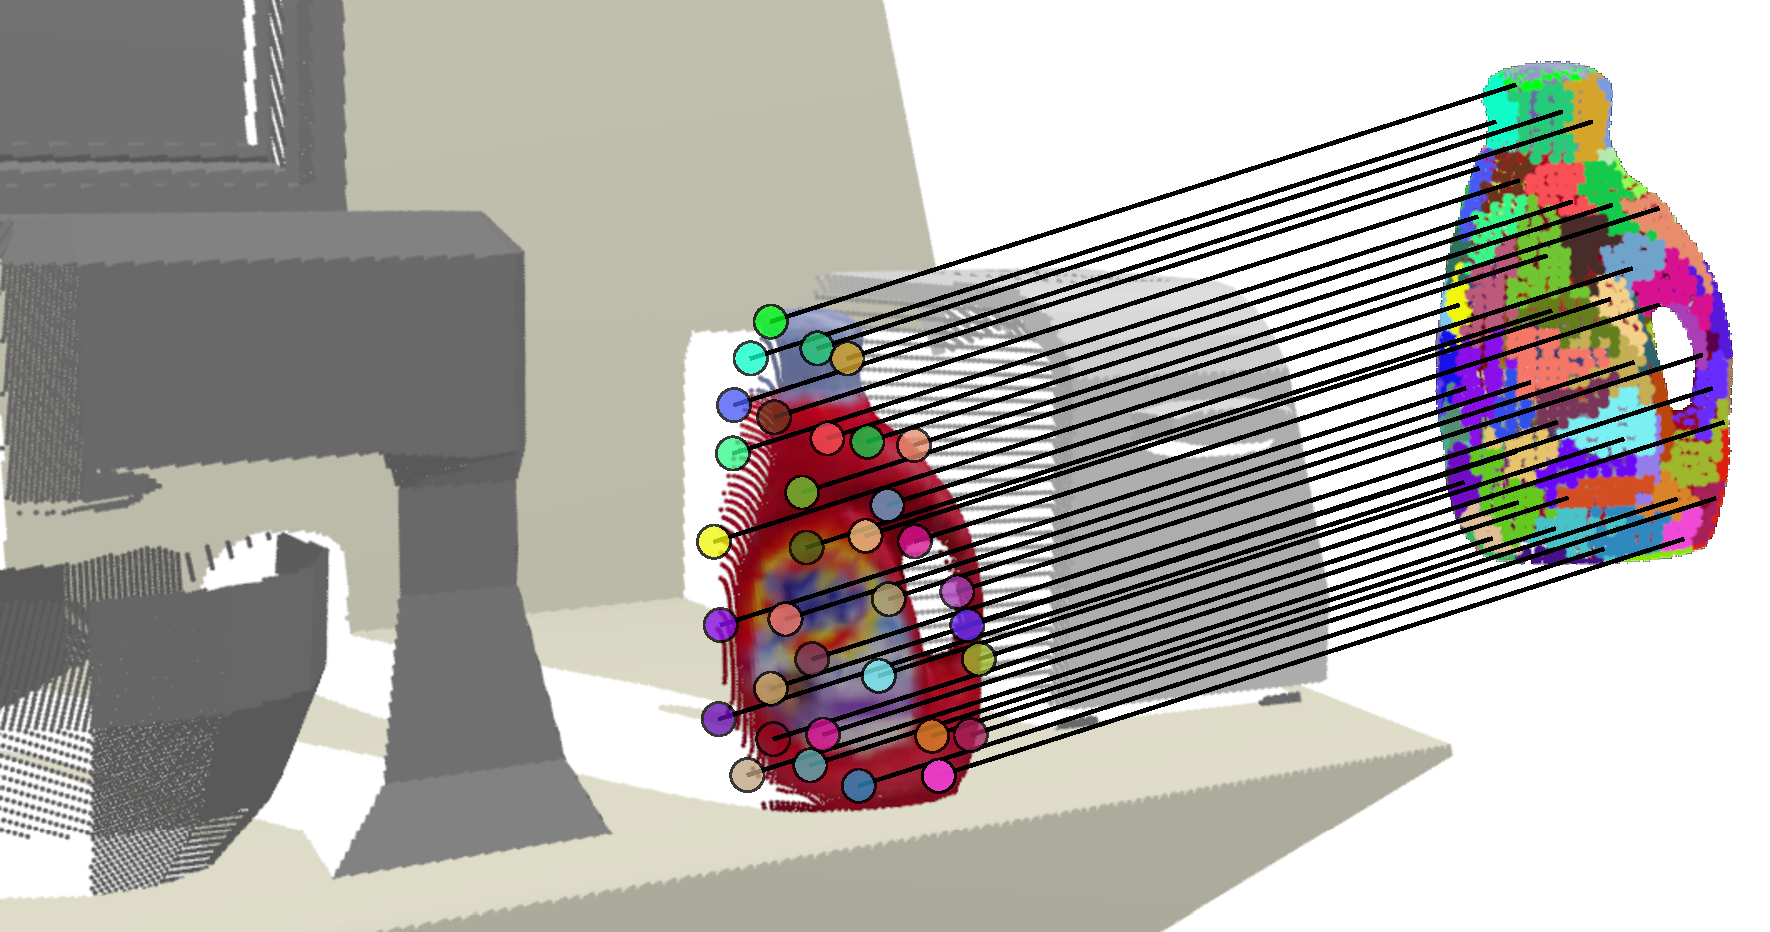
\includegraphics[width=\textwidth]{figures/Tracking/StratifiedCorrespondences.pdf}
  \caption[Stratified Correspondence Matching]{The model is divided into strata (shown as separate colors), and a random point is selected from each stratum for correspondence matching. The colored circles overlaid on the observed point cloud show the search radius used for finding correspondences.}
  \label{fig:Strata}
\end{figure}
While the tracking methodology discussed above works, in practice its run time performance is very poor, even for single objects. Moreover, speed of tracking is highly dependent on the size of object models as well as voxel resolution used. To address this, we propose a sampling scheme which selects a limited number of points from the model to transform and test. By doing this, we achieve linear asymptotic time complexity for the particle filter with respect to the number of particles - there is no dependence on the number of points in the models or the voxel resolution used. The only step which is dependent on the number of input points is the KD-tree construction, but this is only done once for the world model independent of the number of trackers, and must be done as a pre-processing step anyway for normal computation.

The proposed sampling scheme is as follows. We select a spatial sampling resolution $R_{seed}$ based on the number of desired sample points per particle $N_s$. We then divide the model into strata, where each stratum is a supervoxel using the \gls{vccs} method described previously \cite{VCCS_Papon_2013}. Supervoxels are a voxel-based surface patch representation that use connectivity, colors, and normals so that their edges conform well to object part boundaries. The strata are evenly divided over the spatial structure of the model, as seen in Figure~\ref{fig:ModelExample}. Additionally, using supervoxels as the strata ensures that we sample the important features of the models - for example in the model of Figure~\ref{fig:ModelExample}, we have a stratum for the brand logo, as well as ones for the concavities of the handle. 

For each particle, we randomly select a point from each stratum using uniform sampling, and then transform and score it as described in the previous Section. As an additional step, we also select $\frac{N_s}{4}$ points uniformly from the entire model. Using strata reduces the noise which occurs when sampling from the whole model exclusively, while sampling randomly from the entire distribution improves occlusion performance. 

While sampling will tend to produce noisier tracking results for low $N_s$, it also greatly reduces the computational complexity, as we only need to transform and test a small subset of the model points. This allows one to greatly increase the number of particles for a given frame-rate. Importantly, each particle is testing a separate random subset of model points. This results in the product of $N_s$, the number of sample points per particle, and $N$, the number of particles, reaching a critical level where coverage becomes sufficient that error is equivalent to sampling all points. In the results presented below, we shall demonstrate that this critical level can be used to significantly decrease run time for a given level of error. That is, we shall show that the number of points that must be tested overall, for a given level of error, is lower when stratified sampling is used. This means that we can significantly increase accuracy for a given frame-rate, reducing run-time complexity to the point that we can track 6 DoF pose for multiple objects in real-time.   

\section{Experimental Results}
\label{sec:ExperimentalResults}
In this Section we first present results on a set of synthetic videos to quantify the effect of the stratified sampling, and compare results to a state of the art GPU particle filter \cite{Choi_IROS2013}. We then present qualitative results on real videos in a robotic learning application, where we track multiple interacting targets with significant occlusions. In both synthetic and real cases, input consists of RGB-D sequences. Trackers were initialized using an external pose - in the synthetic case, from ground truth, and in the real case, using a pose estimation algorithm \cite{Buch_CVPR2014}. Object models were generated by registering multiple views of the objects using the same RGB-D sensor employed for tracking. All experiments were performed on a standard desktop computer (Intel i7 3.2Ghz), using all four available cores.

\subsection{Results on Synthetic Sequences}
In our first experiment, we demonstrate the effectiveness of our stratified sampling strategy using four synthetic tracking videos from \cite{Choi_IROS2013}. These RGB-D sequences are set in a virtual kitchen (see Figure \ref{fig:KinectBoxMontage}) and each contain a single item to track as the camera moves. Ground truth trajectories of the cameras are given in Figures \ref{fig:PlotsKinectBox}-\ref{fig:PlotsTide}; one can observe that the trajectories are complex, consisting of large variations in position, orientation, and velocity.  

\begin{figure*}[!ht]
  \centering
  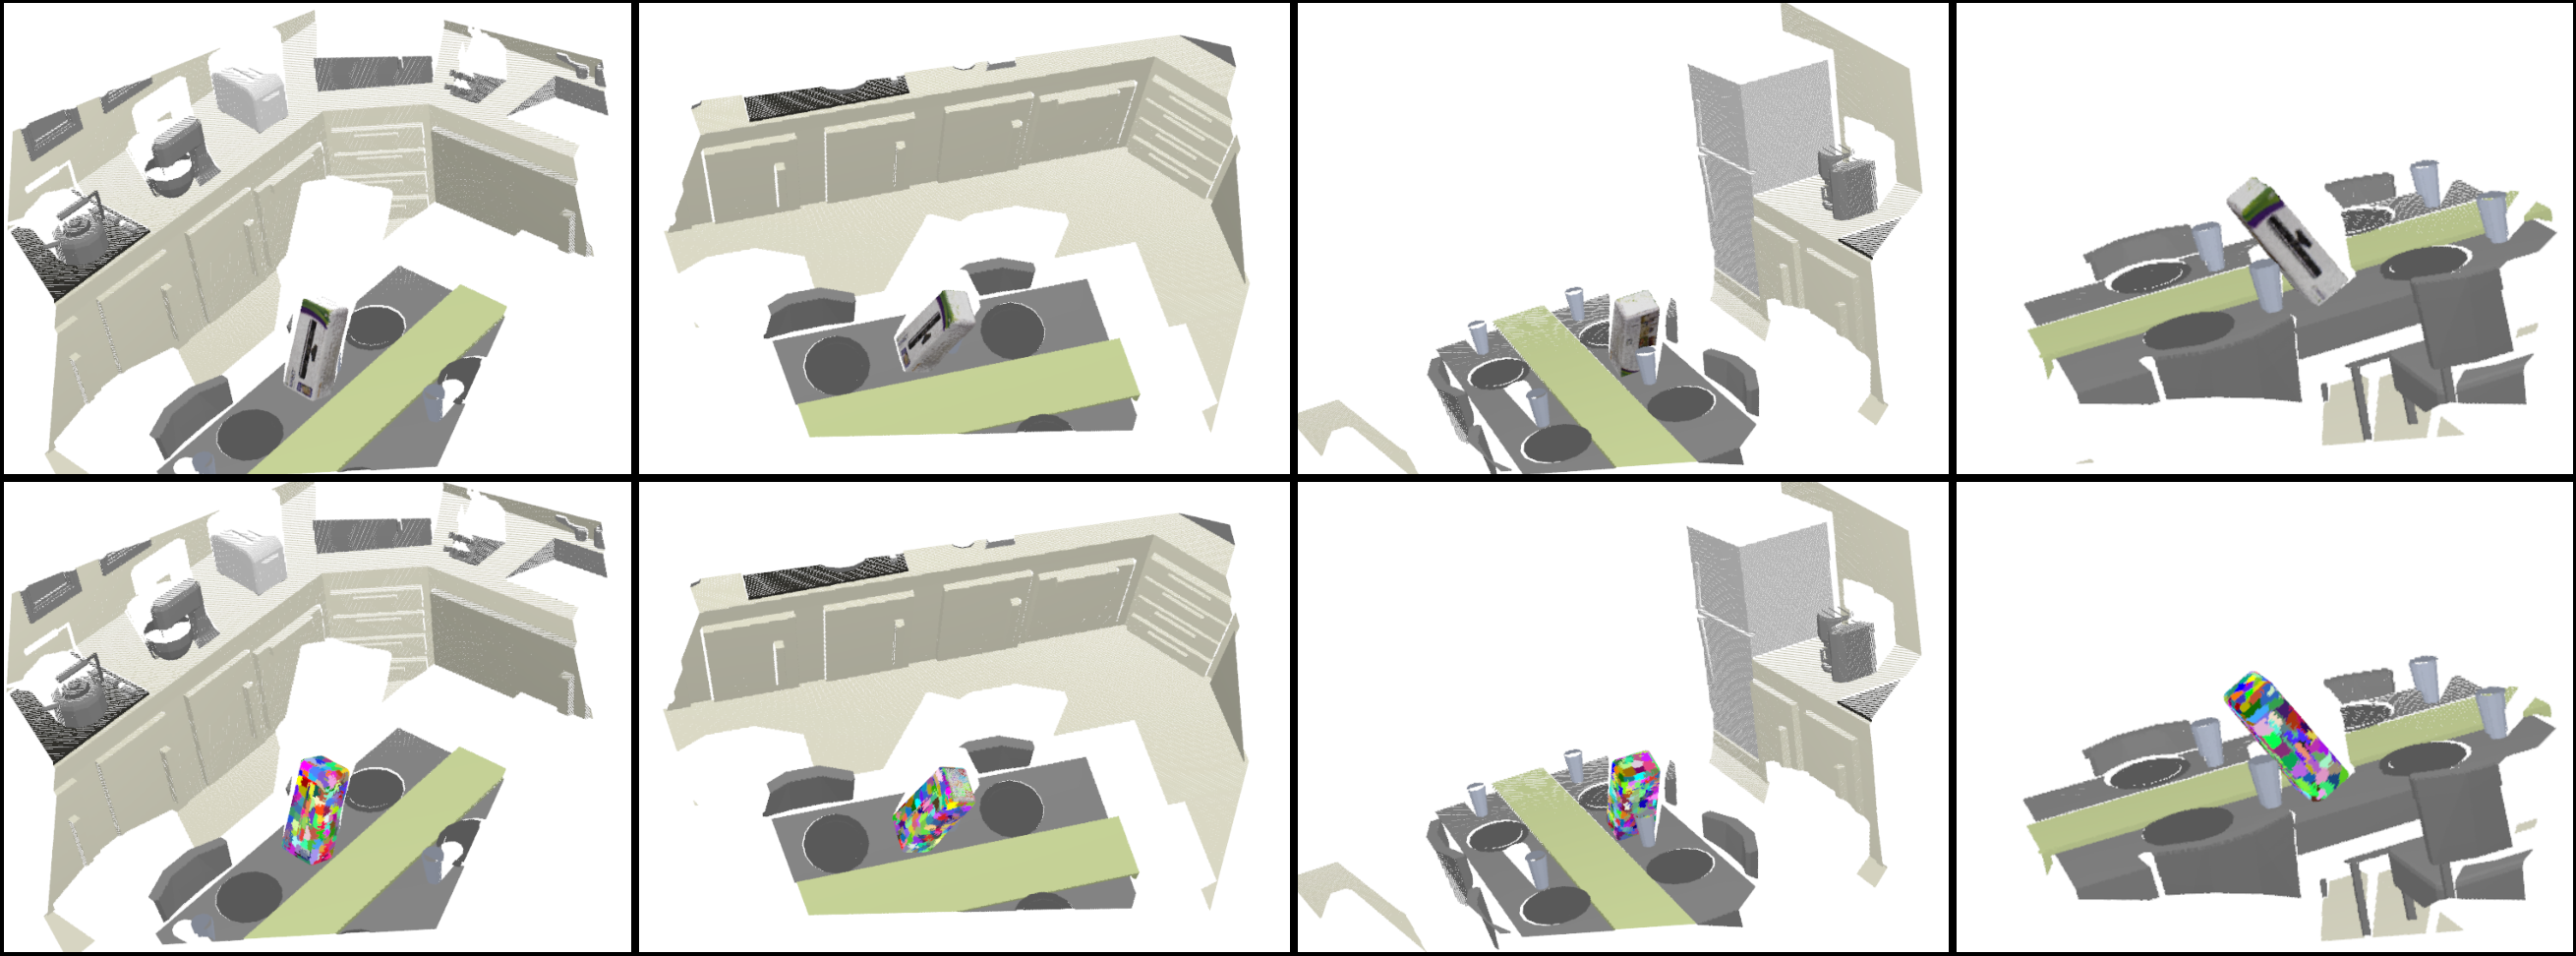
\includegraphics[width=\linewidth]{figures/Tracking/KinectBoxSVMontage.pdf}
  \caption[Tracking on the artificial ``Kinect Box'' sequence.]{Tracking on the artificial ``Kinect Box'' sequence. The top row shows tracked output overlaid on input data, while the bottom row shows the supervoxel strata that are used for sampling.}
  \label{fig:KinectBoxMontage}
\end{figure*}

\missingfigure{Should I add montage of other 3 sequences?}

To evaluate our approach, we compute root mean square (RMS) error in both translation and orientation, averaged over 25 test runs for each sequence. Computation times are measured in ms per frame, and are also averaged across all frames of the 25 test runs. In order to compare with \cite{Choi_IROS2013}, we have combined their RMS error results for each dimension (x, y, z, roll, pitch, yaw) into two measurements - displacement and rotation. Rotation is calculated using the unit quaternion distance metric \cite{Kuffner_ICRA2004}, which is equivalent to the angular distance on the unit sphere. This combination reduces the amount of data to compare without loss, as the choice of orientation of the dimensions is arbitrary and without import. Example displacement and rotation ground truths for the ``Kinect Box'' sequence can be found in Figure \ref{fig:Plots}.

Timing results are given in Figures \ref{fig:ErrorPlotsKinectBox} -\ref{fig:ErrorPlotsTide}, showing results for the four sequences, with each plot scanning across number of particles and number of sample points. Results for all four sequences are similar. One can observe that, for a given level of sampling, the RMS error decreases for both displacement and rotation as the number of particles increases. More importantly, it is also apparent that, for a given level of error, run-time per frame can be minimized by reducing the number of samples used and increasing the number of particles. Additionally, one can observe that RMS error appears to be asymptotic, with lower sampling levels approaching the asymptote at lower run-times.

We should also note that the minimum error asymptote observed is likely a consequence of the sampling resolution of the synthetic Kinect camera. For example, in the ``Kinect Box'' sequence, average distance to neighboring points (8-neighborhood) on the tracked box surface is 3.3 mm. This corresponds almost exactly to our observed error asymptote. This can be observed in all four sequences - our minimal error corresponds closely to the average point to point resolution of the observations on the model. 



%Before we present results on real data, we shall first quantify tracker performance using \gls{vr} data. \gls{vr} data is primarily useful because it allows us to easily obtain accurate ground-truth data for object tracks and poses - something that is generally not possible with real data \cite{Rossmann2012d}. With this in mind we have developed a \gls{vr} setup and benchmark \cite{VR_Benchmark_Paper} which simulates the platform we shall use in the real data shown later. The virtual platform has many simulated cameras, but in these tests we use two simulated Kinect RGB-D sensors with overlapping fields of view covering the entire work area. The sensor simulation can generate benchmark images and point clouds with controlled levels of quality, from ``ideal'' to ``real''. \footnote{Here, ``real'' is defined by the similarity of outcomes when real and simulated data are processed by libraries such as OpenCV and PCL, e.g. color histograms (RGB deviation, RGB saturation), edge detection, SURF feature detection and RANSAC feature similarity.} In the following tests we used the standard depth error of the Kinect as our lowest noise level and compared the algorithms with less accurate testdata.

%Once again, our benchmarking task is assembly of the well-established ``Cranfield'' set \cite{Collins1985,Schou2012,Martinez2014} (see Fig. \ref{fig:cad_models}).The actual assembly actions in \gls{vr} are carried out and tracked with a data-glove, generating accurate, objective ground-truth data, e.g. exact object positions as well as detailed information on the timing and existence of object manipulations and spatial relations between manipulated objects. Comparisons of real and virtual images were made in the project FastMap \cite{Rossmann2012b} and showed that artificial and real images led to very similar result in computer vision algorithms. 

%In our first experiment, we demonstrate the effectiveness of our stratified sampling strategy. We used a simple scenario in which we must track two bolts as they are picked up and inserted into a faceplate. To simplify the analysis, we fix the run-time variable by setting a desired frame-rate of 20fps \footnote{All these experiments were run on the same machine - an i7 980x with 32g of memory}, and then determined experimentally the number of particles for which this frame rate was sustainable at different degrees of sampling. Degree of sampling is simply the ratio of the number of points sampled to the number of points present in the model, $\frac{N_s}{N_m}$. Table \ref{table:timing} gives the average frame rates and standard deviation measured during the runs. Figure \ref{TODOFIGURE} shows average error rates for the different degrees of sampling. Additionally, Figure \ref{TODOFIGURE} shows the affect on error and run time of increased particle number for fixed degrees of sampling. Finally, Figure \ref{fig:CombinedNoNoise} gives an example of what the tracked output looks like versus ground truth - it is evident that the tracker is able to follow the objects quite well in terms of translation. Rotations, on the other hand, are much noisier, due to the rotational symmetries present in the tracked object (the bolt).  

%%%%%%%%%%%%%%%%%%%%%%%%%%%%%%%%%%%%%%%%%%%%%%%%%%%%%%%%%%
\begin{figure*}[!ht]
  \centering
  \subfloat{{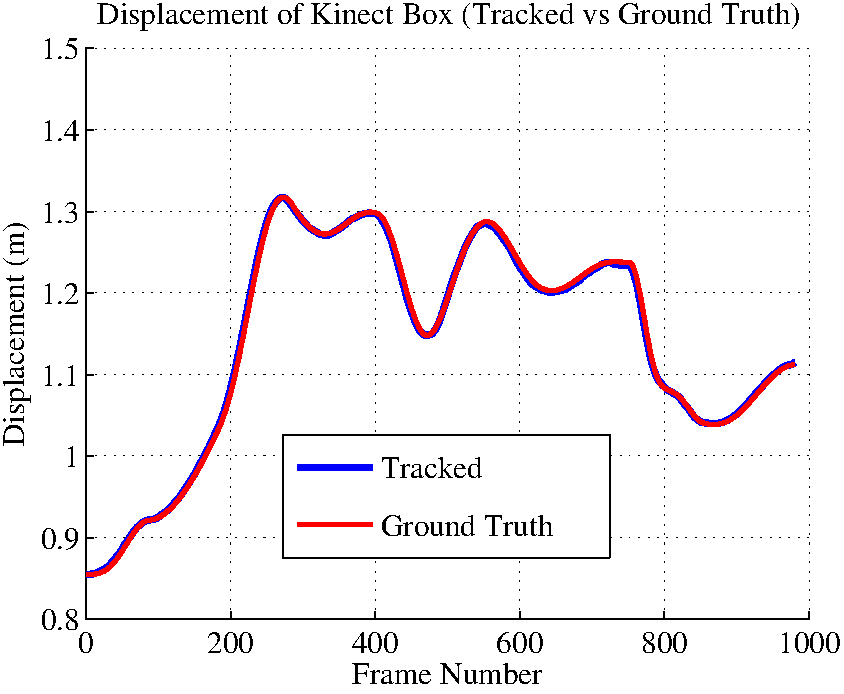
\includegraphics[width=.46\textwidth]{figures/Tracking/ErrorComps/DispKinectBox.pdf} }} %
  \qquad
  \subfloat{{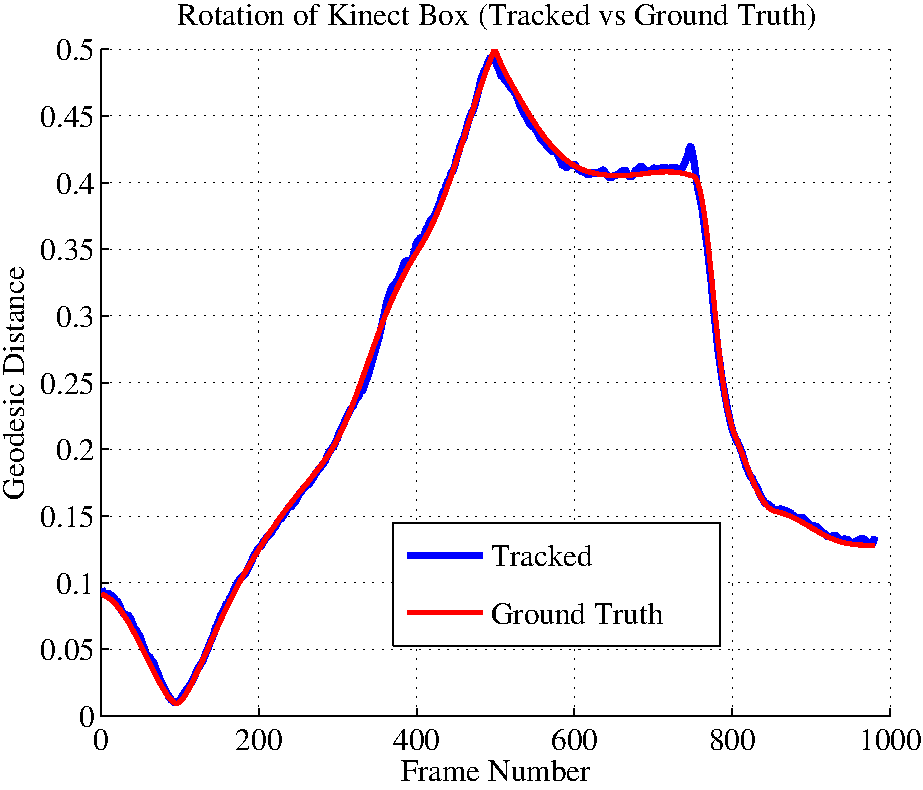
\includegraphics[width=.46\textwidth]{figures/Tracking/ErrorComps/AngleKinectBox.pdf} }}%
  \caption[Tracked vs Ground Truth - Kinect Box]{Displacement and rotation ground truth, with an example tracked result from a single run at $N_{samples}=100$ and $N_{particles}=1000$ (a frame rate of 20 fps).}%
  \label{fig:PlotsKinectBox}%
\end{figure*}

\begin{figure*}[!ht]
  \centering 
  \vspace{-10pt}
  \subfloat{{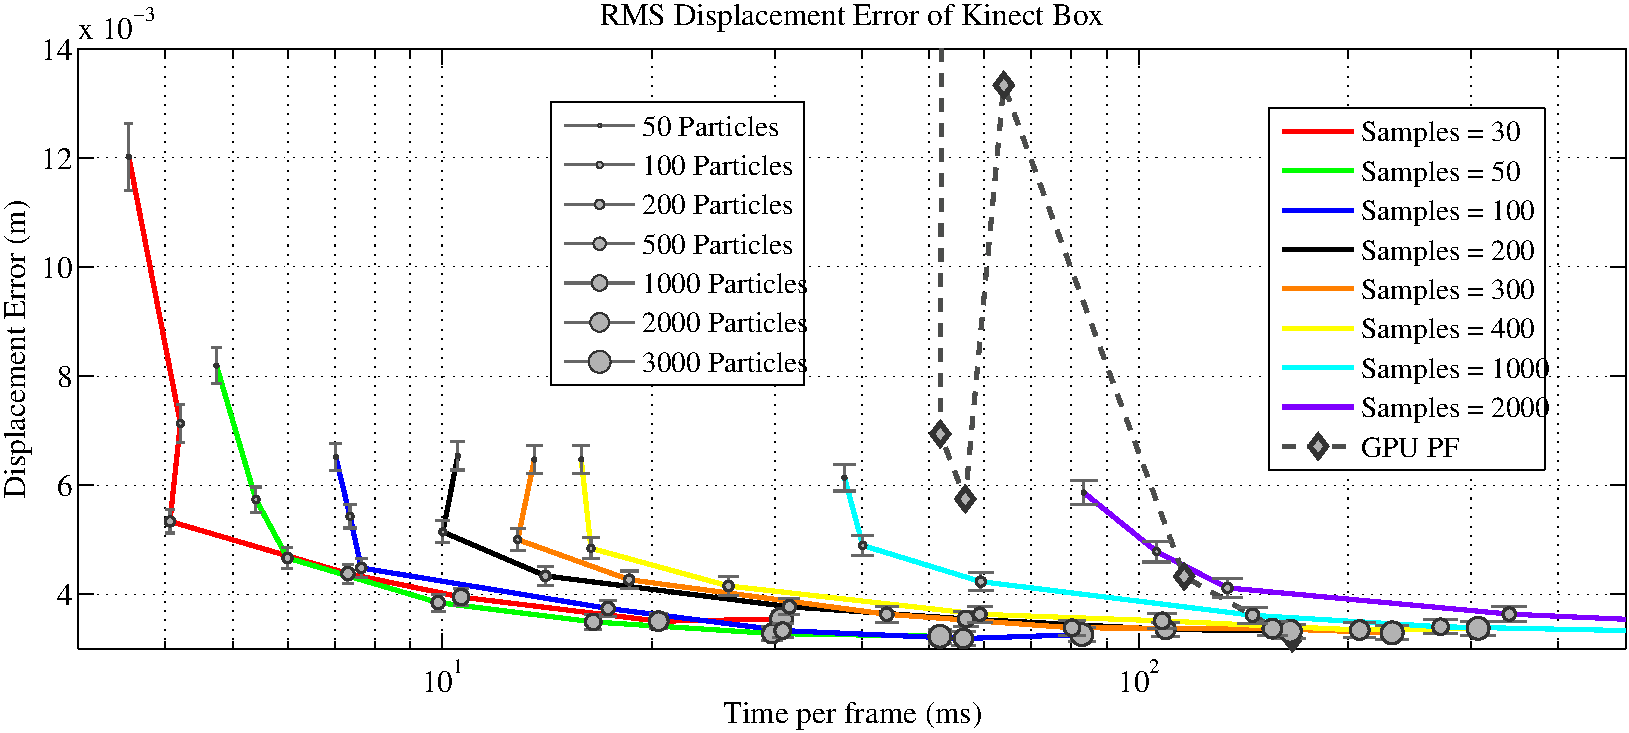
\includegraphics[width=0.98\linewidth]{figures/Tracking/ErrorComps/DispErrorKinectBox.pdf} }} \\
  \vspace{-10pt}
  \subfloat{{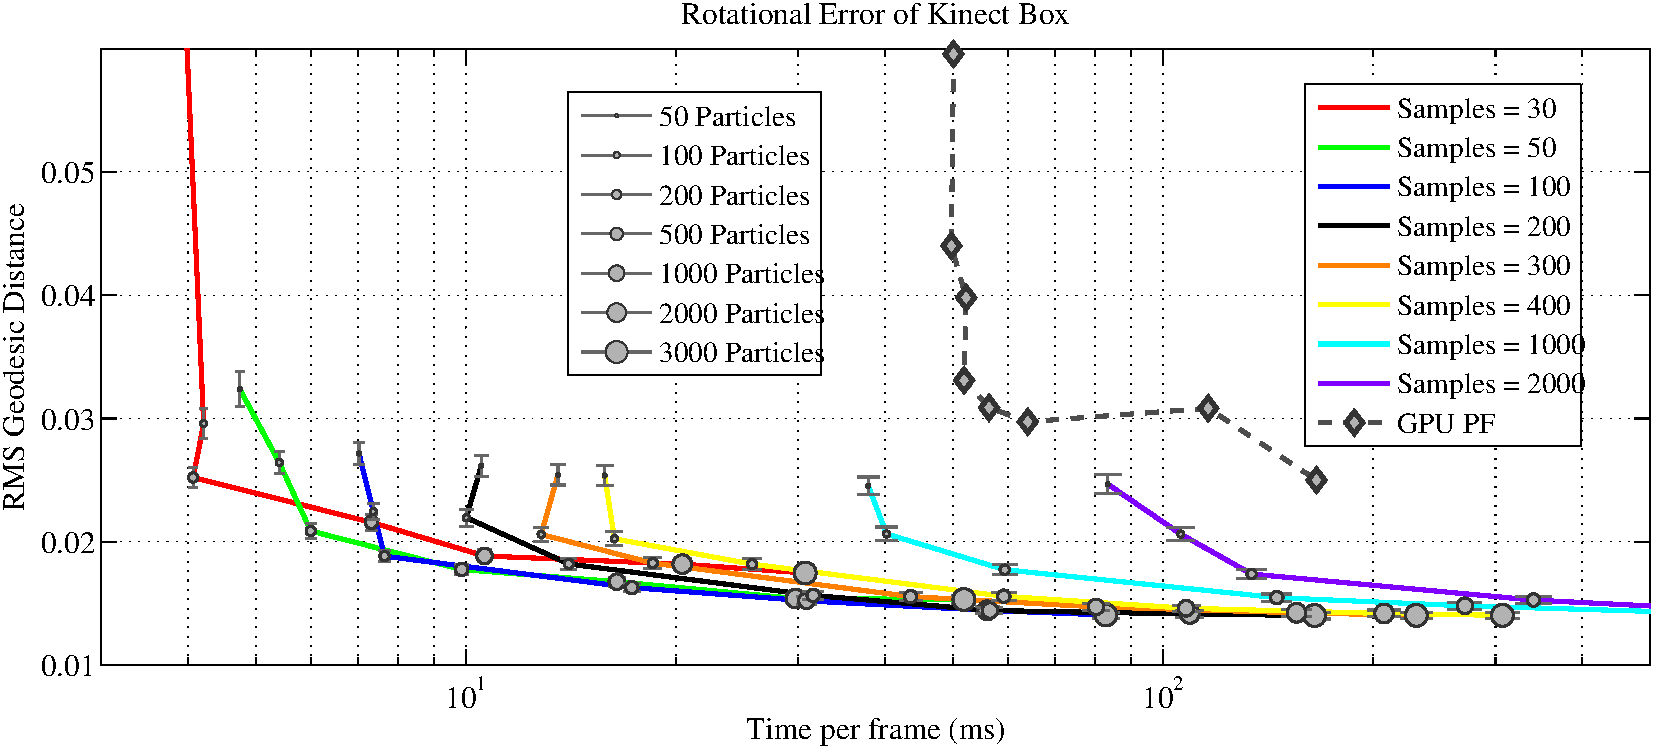
\includegraphics[width=1.0\linewidth]{figures/Tracking/ErrorComps/AngularErrorKinectBox.pdf} }}   \vspace{-7pt} \\
  \caption[Results on the Kinect Box artificial sequence.]{Results on the Kinect Box artificial sequence. Each colored curve represents a certain number of samples, and gives mean RMS error averaged over 25 trial runs for increasing numbers of particles.}%
  \label{fig:ErrorPlotsKinectBox}%
\end{figure*}
%%%%%%%%%%%%%%%%%%%%%%%%%%%%%%%%%%%%%%%%%%%%%%%%%%%%%%%%%%
\begin{figure*}[!ht]
  \centering
  \subfloat{{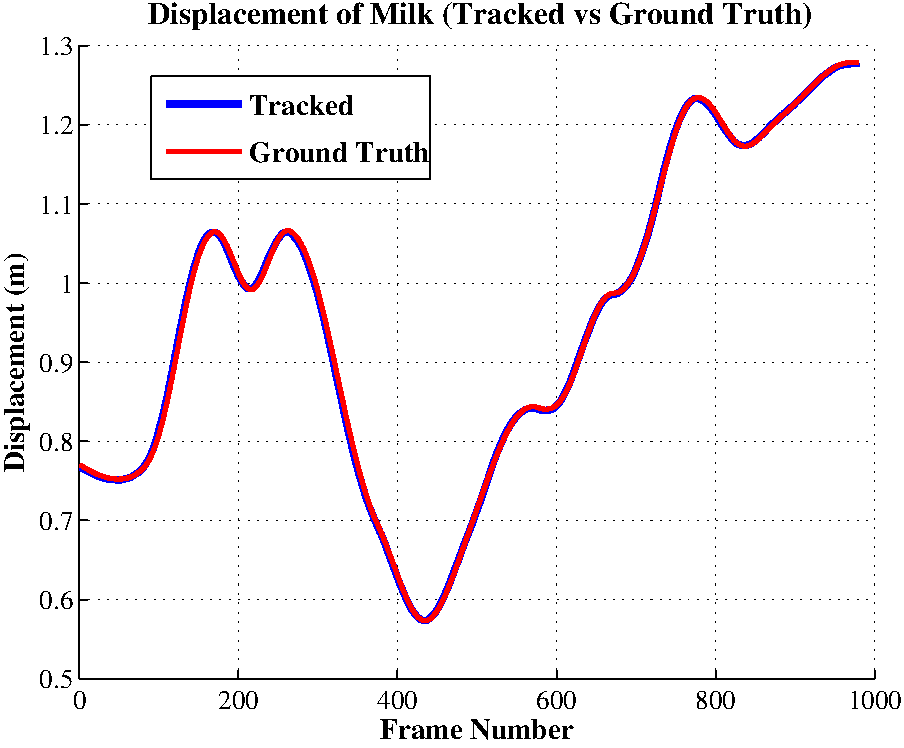
\includegraphics[width=.46\textwidth]{figures/Tracking/ErrorComps/DispMilk.pdf} }} %
  \qquad
  \subfloat{{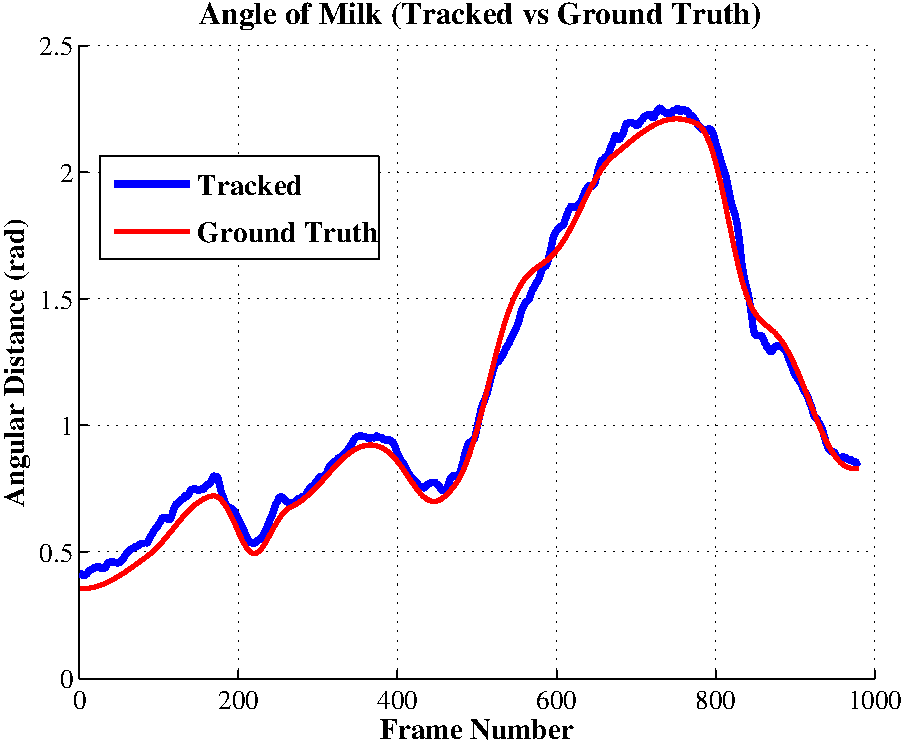
\includegraphics[width=.46\textwidth]{figures/Tracking/ErrorComps/AngleMilk.pdf} }}%
  \caption[Tracked vs Ground Truth - Milk]{Displacement and rotation ground truth, with an example tracked result from a single run at $N_{samples}=100$ and $N_{particles}=1000$ (a frame rate of 20 fps).}%
  \label{fig:PlotsMilk}%
\end{figure*}

\begin{figure*}[!ht]
  \centering 
  \vspace{-10pt}
  \subfloat{{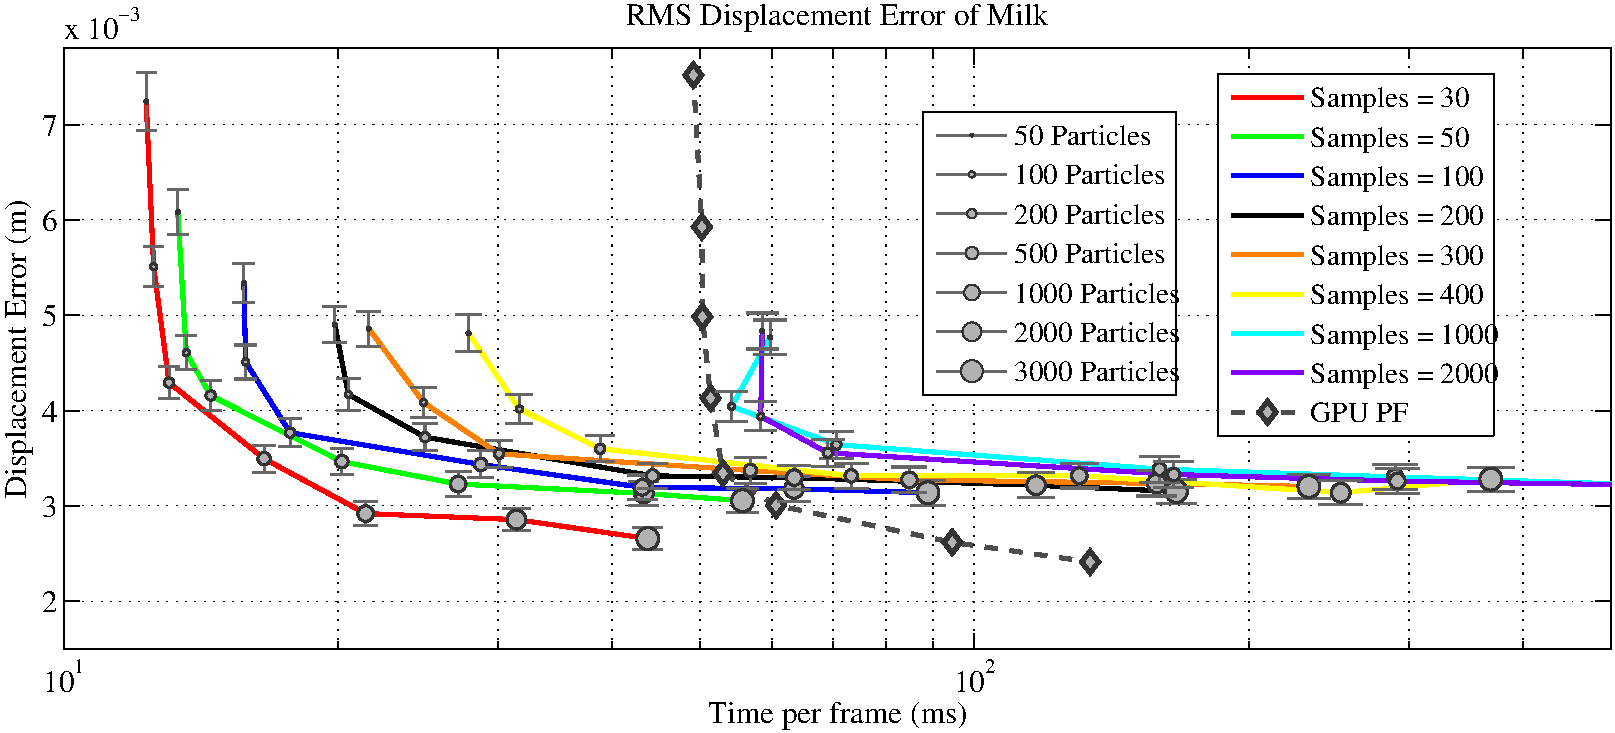
\includegraphics[width=0.98\linewidth]{figures/Tracking/ErrorComps/DispErrorMilk.pdf} }} \\
  \vspace{-10pt}
  \subfloat{{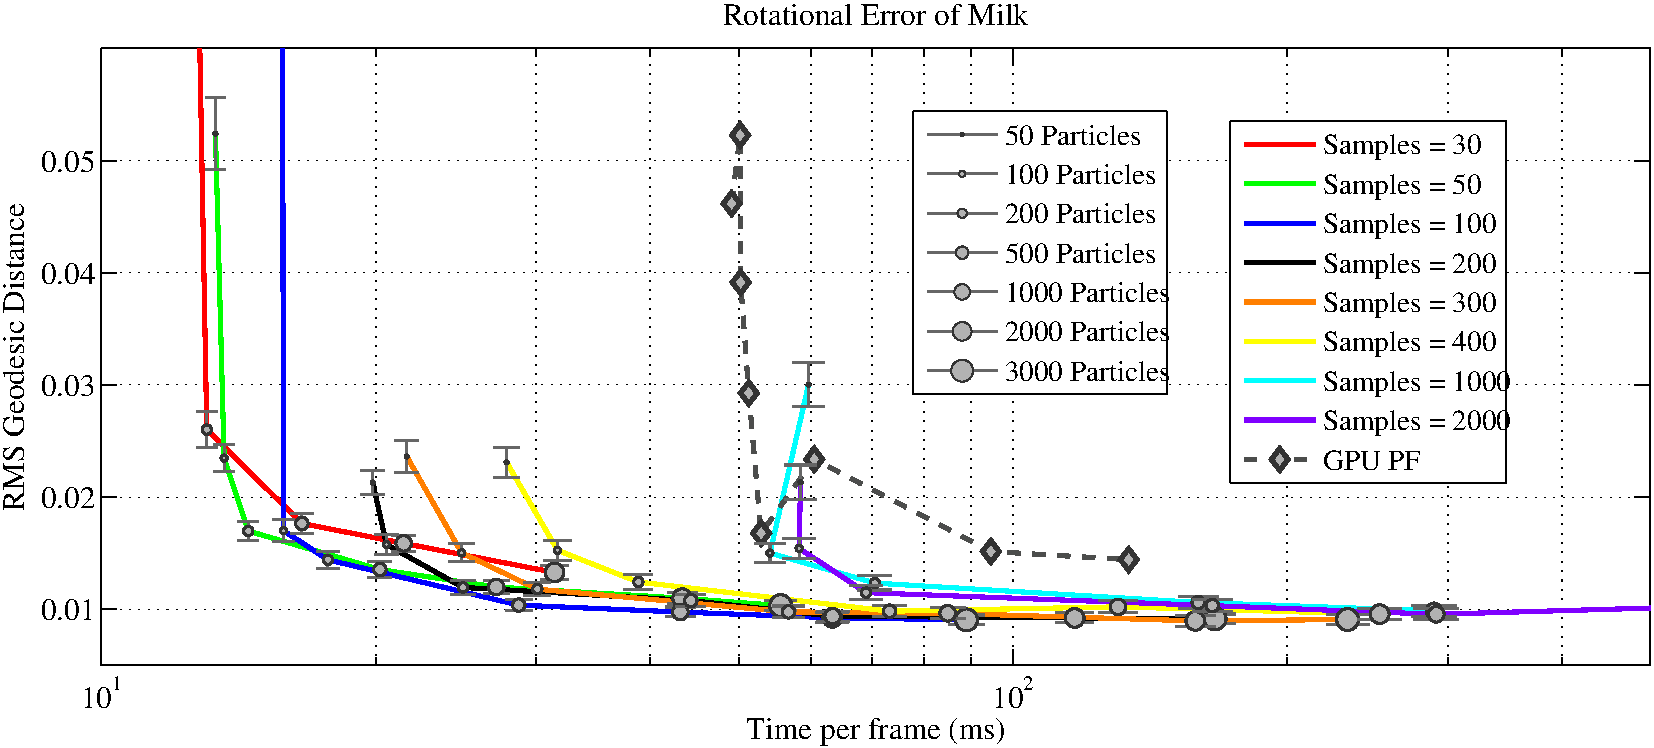
\includegraphics[width=1.0\linewidth]{figures/Tracking/ErrorComps/AngularErrorMilk.pdf} }}   \vspace{-7pt} \\
  \caption[Results on the Milk artificial sequence.]{Results on the Milk artificial sequence. Each colored curve represents a certain number of samples, and gives mean RMS error averaged over 25 trial runs for increasing numbers of particles.}%
  \label{fig:ErrorPlotsMilk}%
\end{figure*}
%%%%%%%%%%%%%%%%%%%%%%%%%%%%%%%%%%%%%%%%%%%%%%%%%%%%%%%%%%
\begin{figure*}[!ht]
  \centering
  \subfloat{{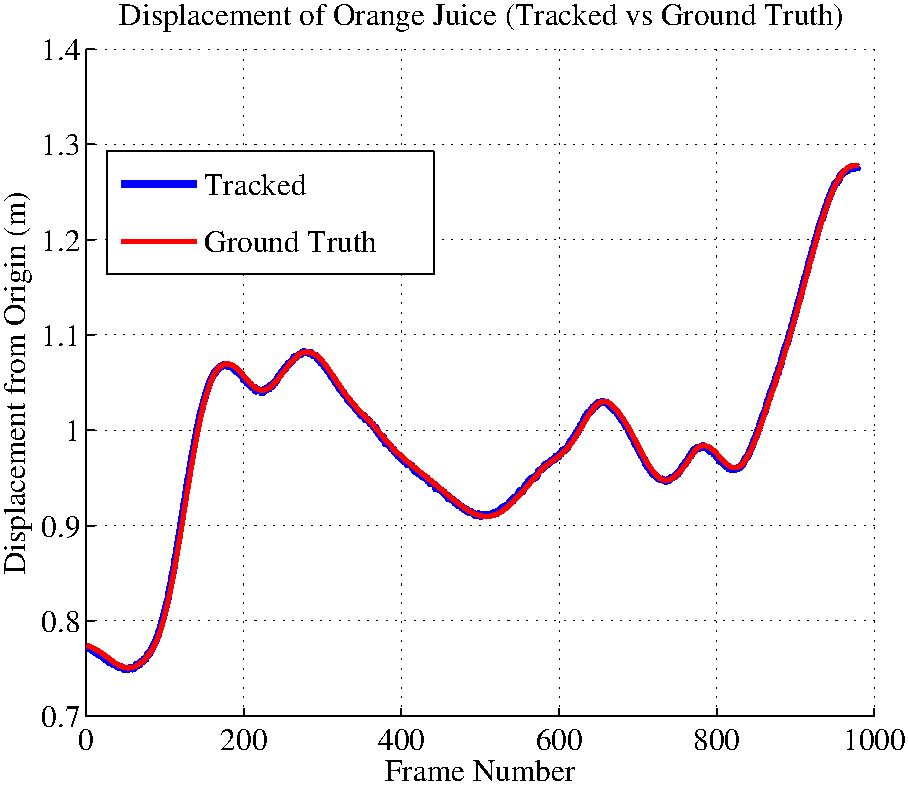
\includegraphics[width=.46\textwidth]{figures/Tracking/ErrorComps/DispOrangeJuice.pdf} }} %
  \qquad
  \subfloat{{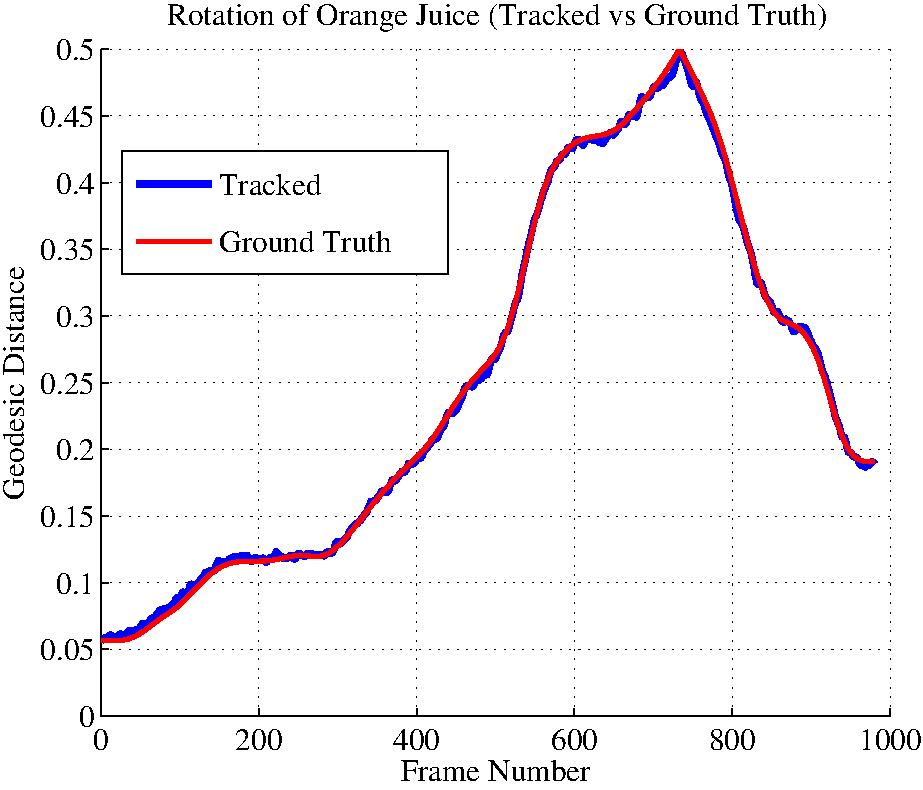
\includegraphics[width=.46\textwidth]{figures/Tracking/ErrorComps/AngleOrangeJuice.pdf} }}%
  \caption[Tracked vs Ground Truth - Orange Juice]{Displacement and rotation ground truth, with an example tracked result from a single run at $N_{samples}=100$ and $N_{particles}=1000$ (a frame rate of 20 fps).}%
  \label{fig:PlotsOrangeJuice}%
\end{figure*}

\begin{figure*}[!ht]
  \centering 
  \vspace{-10pt}
  \subfloat{{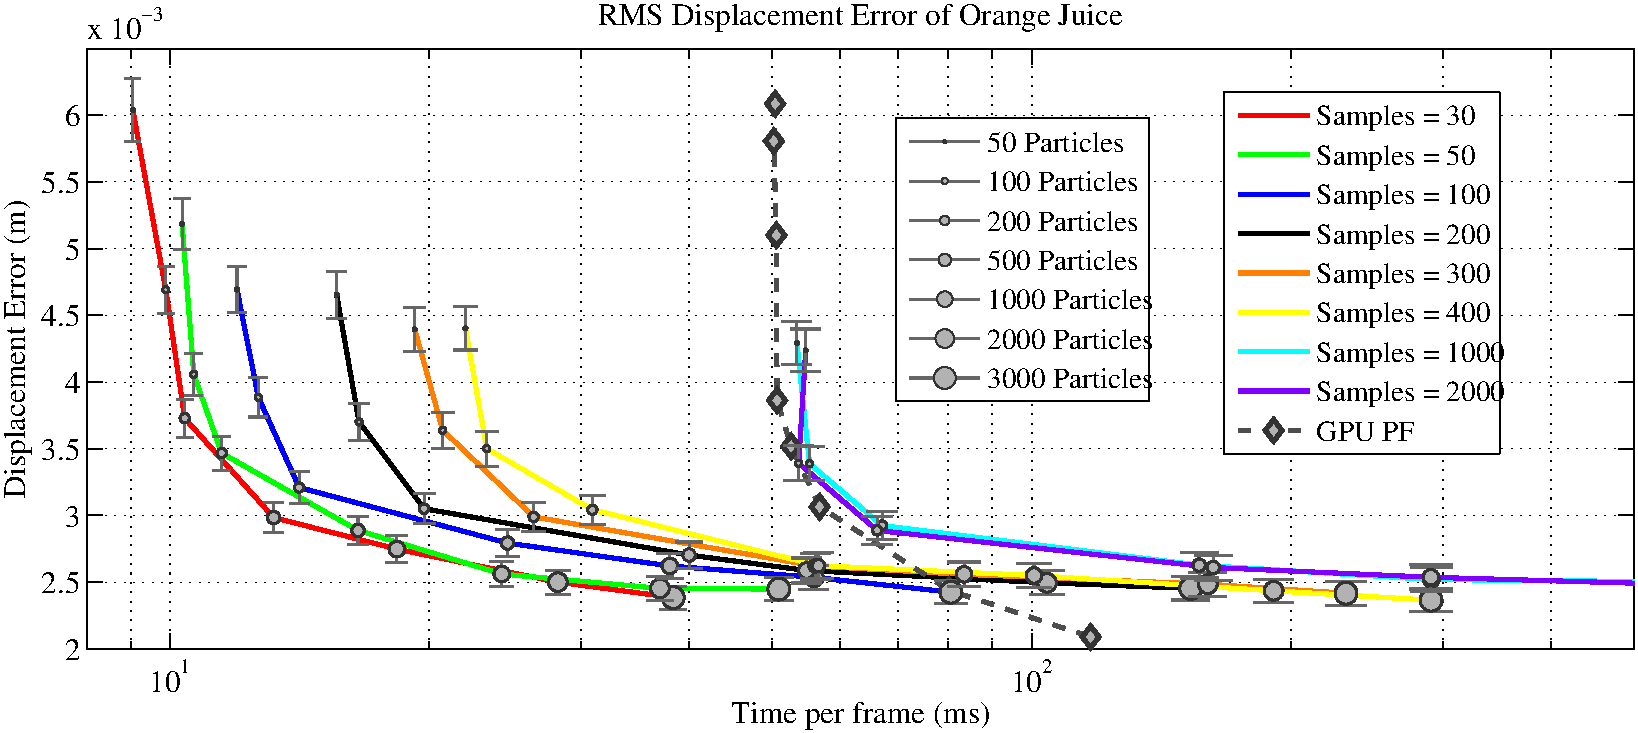
\includegraphics[width=0.98\linewidth]{figures/Tracking/ErrorComps/DispErrorOrangeJuice.pdf} }} \\
  \vspace{-10pt}
  \subfloat{{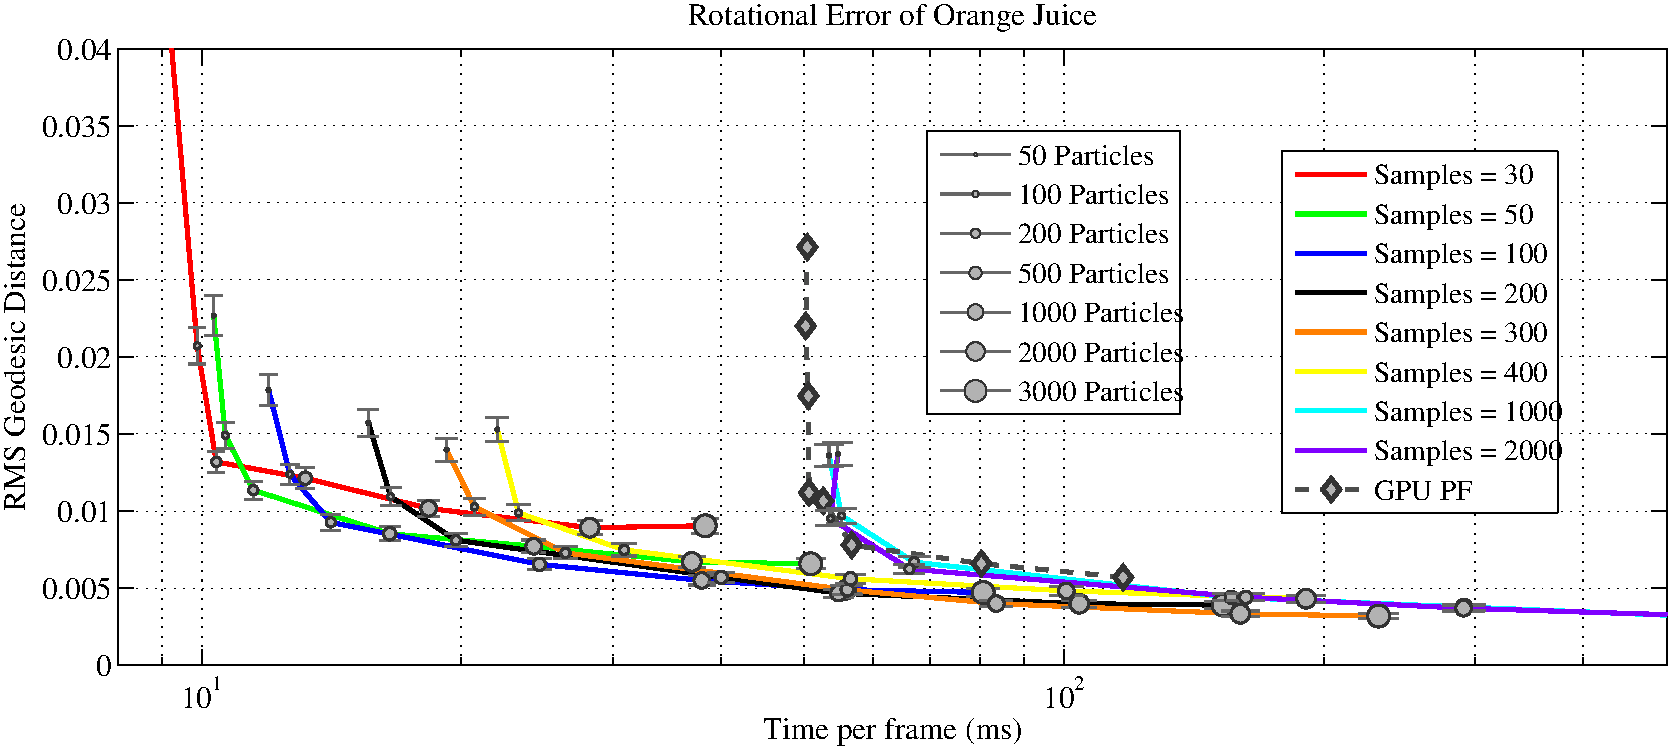
\includegraphics[width=1.0\linewidth]{figures/Tracking/ErrorComps/AngularErrorOrangeJuice.pdf} }}   \vspace{-7pt} \\
  \caption[Results on the Orange Juice artificial sequence.]{Results on the Orange Juice artificial sequence. Each colored curve represents a certain number of samples, and gives mean RMS error averaged over 25 trial runs for increasing numbers of particles.}%
  \label{fig:ErrorPlotsOrangeJuice}%
\end{figure*}
%%%%%%%%%%%%%%%%%%%%%%%%%%%%%%%%%%%%%%%%%%%%%%%%%%%%%%%%%%
\begin{figure*}[!ht]
  \centering
  \subfloat{{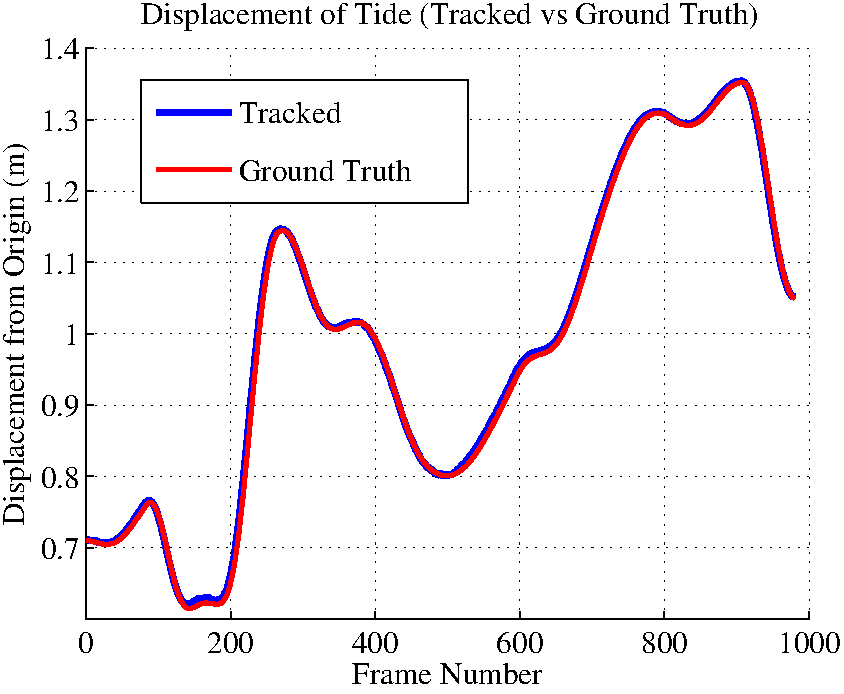
\includegraphics[width=.46\textwidth]{figures/Tracking/ErrorComps/DispTide.pdf} }} %
  \qquad
  \subfloat{{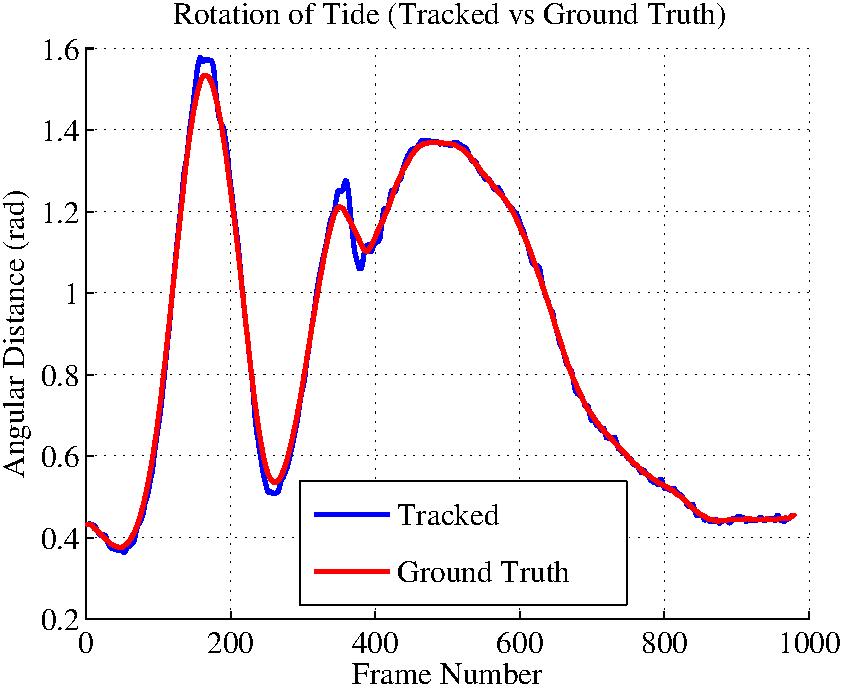
\includegraphics[width=.46\textwidth]{figures/Tracking/ErrorComps/AngleTide.pdf} }}%
  \caption[Tracked vs Ground Truth - Tide]{Displacement and rotation ground truth, with an example tracked result from a single run at $N_{samples}=100$ and $N_{particles}=1000$ (a frame rate of 20 fps).}%
  \label{fig:PlotsTide}%
\end{figure*}

\begin{figure*}[!ht]
  \centering 
  \vspace{-10pt}
  \subfloat{{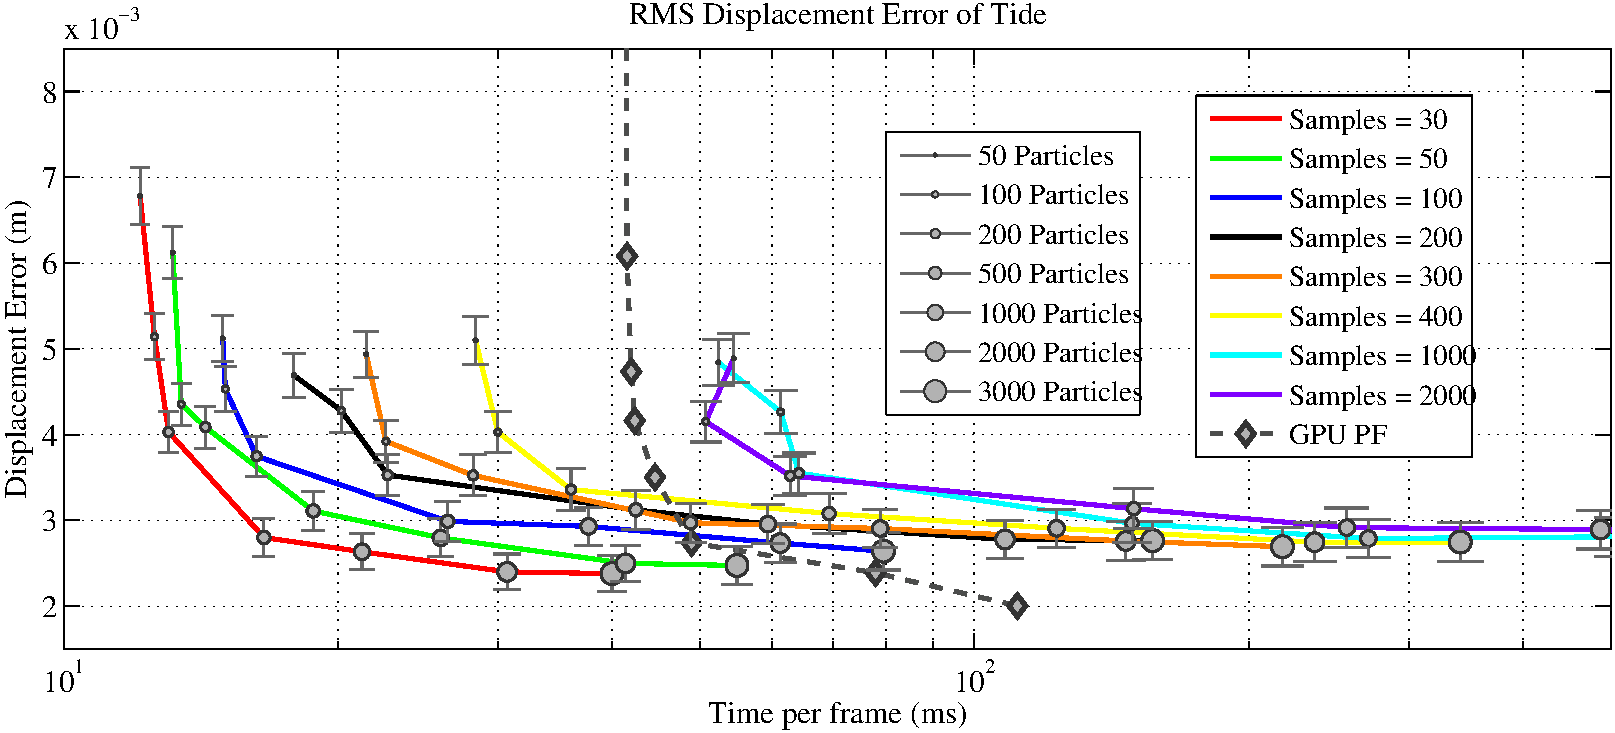
\includegraphics[width=0.98\linewidth]{figures/Tracking/ErrorComps/DispErrorTide.pdf} }} \\
  \vspace{-10pt}
  \subfloat{{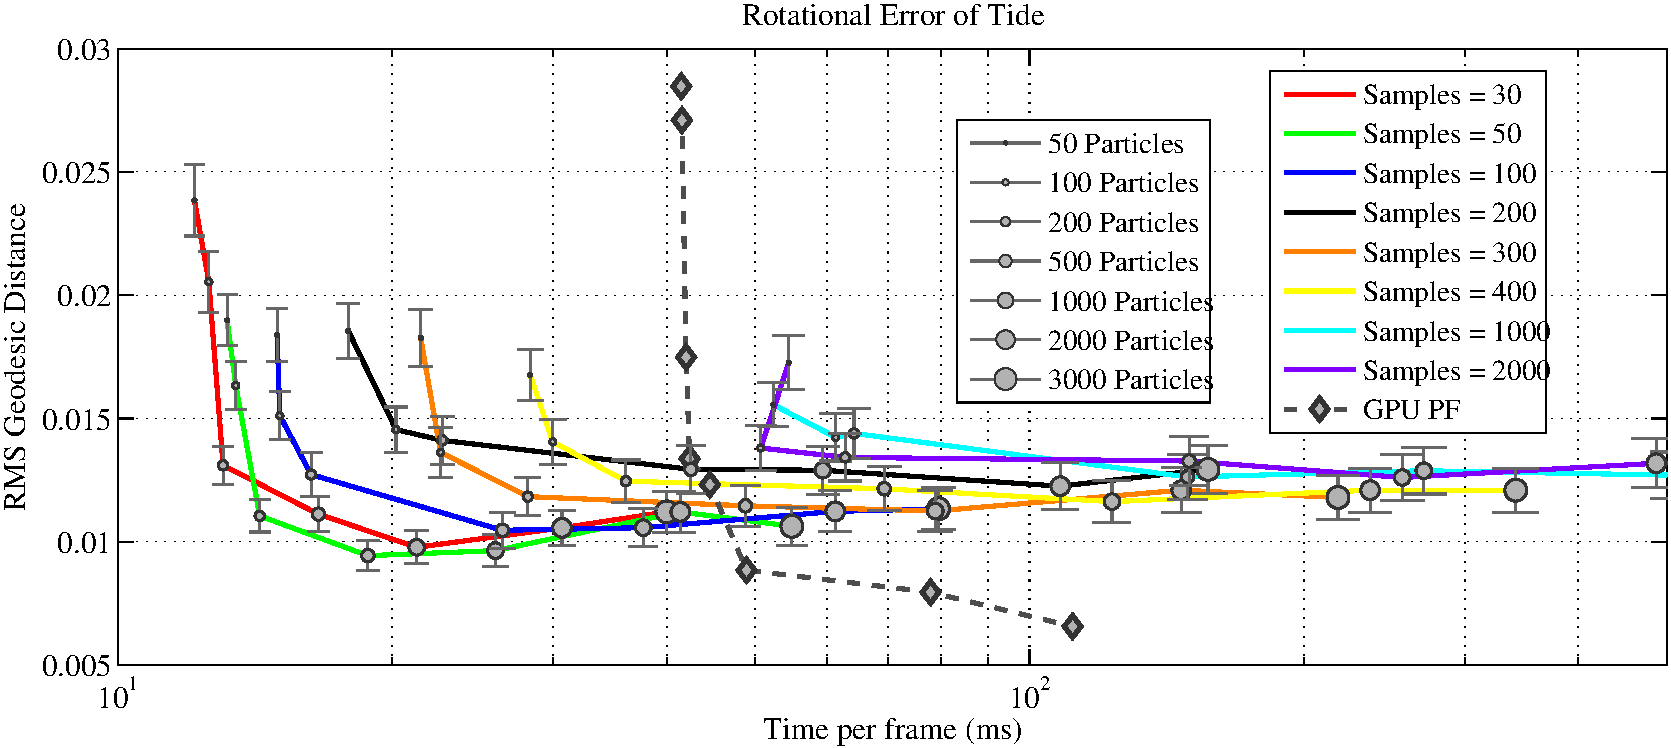
\includegraphics[width=1.0\linewidth]{figures/Tracking/ErrorComps/AngularErrorTide.pdf} }}   \vspace{-7pt} \\
  \caption[Results on the Tide artificial sequence.]{Results on the Tide artificial sequence. Each colored curve represents a certain number of samples, and gives mean RMS error averaged over 25 trial runs for increasing numbers of particles.}%
  \label{fig:ErrorPlotsTide}%
\end{figure*}
%%%%%%%%%%%%%%%%%%%%%%%%%%%%%%%%%%%%%%%%%%%%%%%%%%%%%%%%%%

Our performance compares favorably to the results of Choi and Christensen \cite{Choi_IROS2013} - for a given level of error, we achieve per-frame run times that are between half and a tenth of their published results. Additionally, we consistently reach the error asymptote at considerably lower run times. We should also note that the highest sampling level shown corresponds to a complete sampling of the model, and can be thought of as equivalent to the baseline PCL implementation, although we have made some modifications to the resampling and dynamic model which improve results. As can be seen, we are at least an order of magnitude faster than this base implementation.

\subsection{Results on Real Sequences}
One application of our tracker is to provide semantic understanding and imitation of assembly tasks. This can be accomplished by tracking all interacting parts of an assembly as a human demonstrates, and then using the trajectories and poses in order to train a robot to replicate the construction. Additionally, the tracked output can be used as an input for the robot during construction in order to verify that it has successfully completed each step of the task. 

\begin{figure*}[!ht]
  \centering
  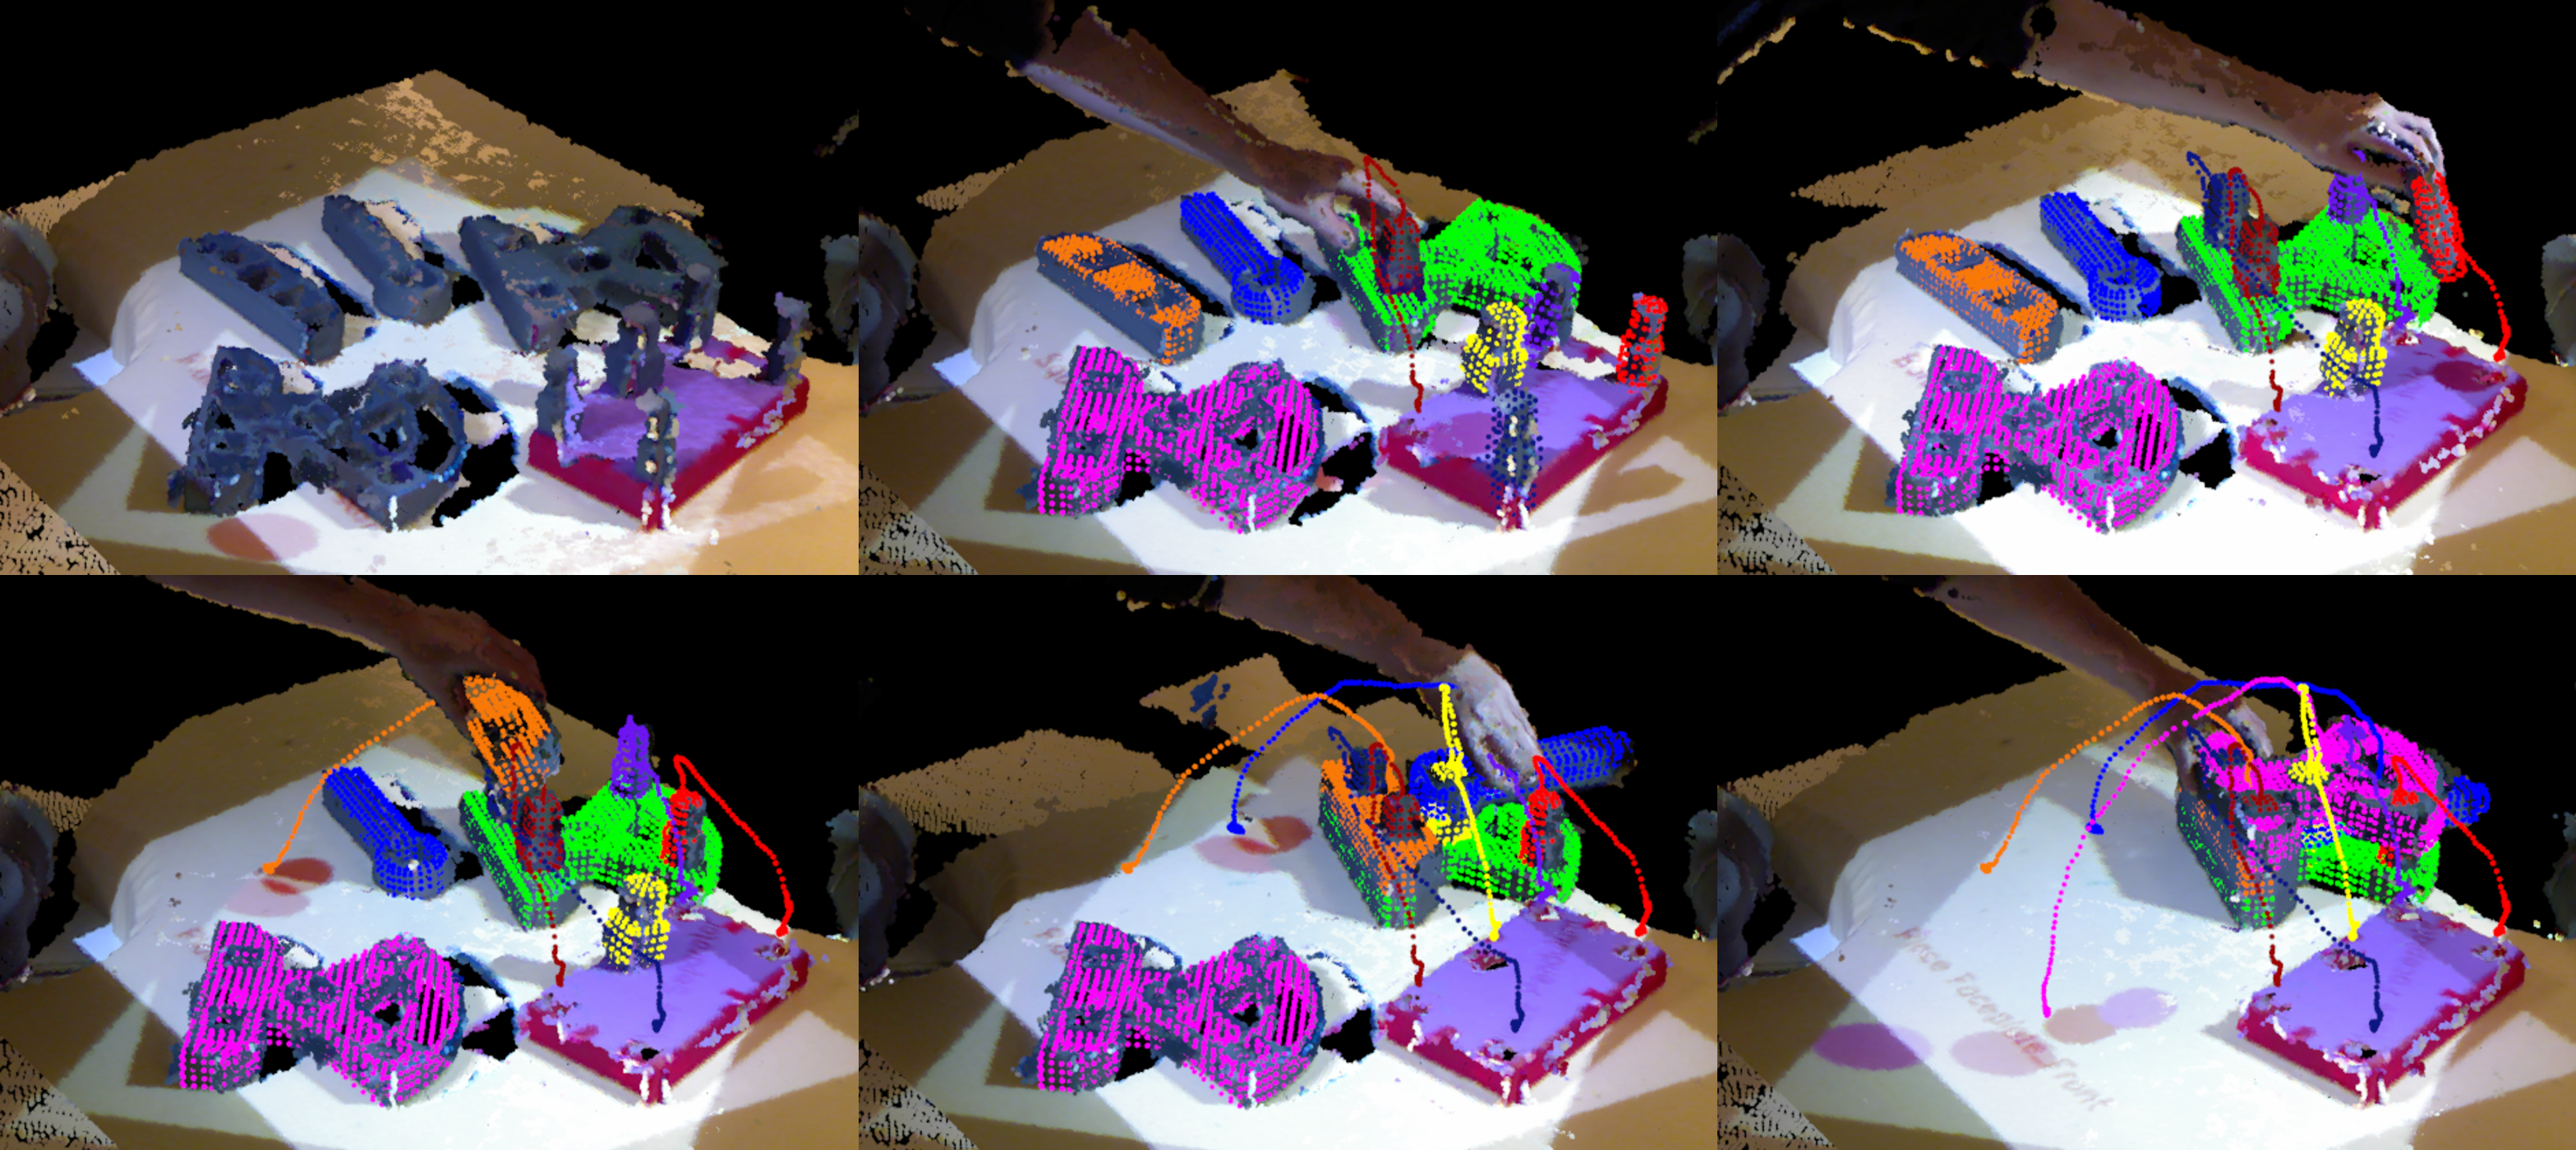
\includegraphics[width=1.0\textwidth]{figures/Tracking/HumanMontageSmall.pdf}
  \caption[Human demonstration of assembly of the Cranfield Scenario.]{Human demonstration of assembly of the Cranfield Scenario. Tracking runs live for all objects at once at sufficient frame rates to track the whole task.}
  \label{fig:Tracking_Montage}
\end{figure*}

As a demonstration of this, we shall once again use the well established ``Cranfield'' benchmark set \cite{Collins1985}, consisting of eight pieces which can be assembled in a number of different orders. In our experiments, models consist of voxelized point clouds derived from high-resolution models of the pieces, and initial poses for tracking are found using a combined object recognition and pose estimation algorithm \cite{Buch_CVPR2014}. Each object is tracked using an independent particle filter, with $N_{samples}$ set to 50, and $N_{particles}$ set to 1000. 

Recordings were made on the MARVIN platform at the University of Southern Denmark, and use 2 Kinect RGB-D cameras \footnote{It is well-known that multiple Kinect sensors sharing a common field of view will cause IR interference, resulting in poor depth reconstructions. A known solution, which the platform incorporates, is the use of vibrating motors mounted on the Kinect sensors \cite{Butler2012}. This method has been shown to effectively blur out the noisy contributions of external sensors, while maintaining a high depth reconstruction quality.}. The recordings were performed by different people, where the people were following assembly instructions presented by the planning system of the IntellAct project. A description of the planner is beyond the scope of this work (we refer the reader to \cite{TODOPLANNER}), but for our purposes we just need to know that the order of assembly varies from sequence to sequence. 

Figure \ref{fig:Tracking_Montage} shows a montage of screenshots captured as a human demonstrates assembly of the benchmark. As can be seen, all pieces are successfully tracked from start to finish, with each tracker outputting smooth trajectories that can be used for training a robot using Dynamic Motion Primitives (DMP) \cite{Kulvicius2012}. In Figure \ref{fig:TrackingResults} we show tracks from multiple different human demonstrations - one can observe the different strategies that people employ in assembling the benchmark. The tracks in the lower right corner of the Figure are from a robot reproducing the assembly after being trained on the human demonstrations \cite{Rossman_ICRA2014}. 

\begin{figure*}[!ht]
  \centering
  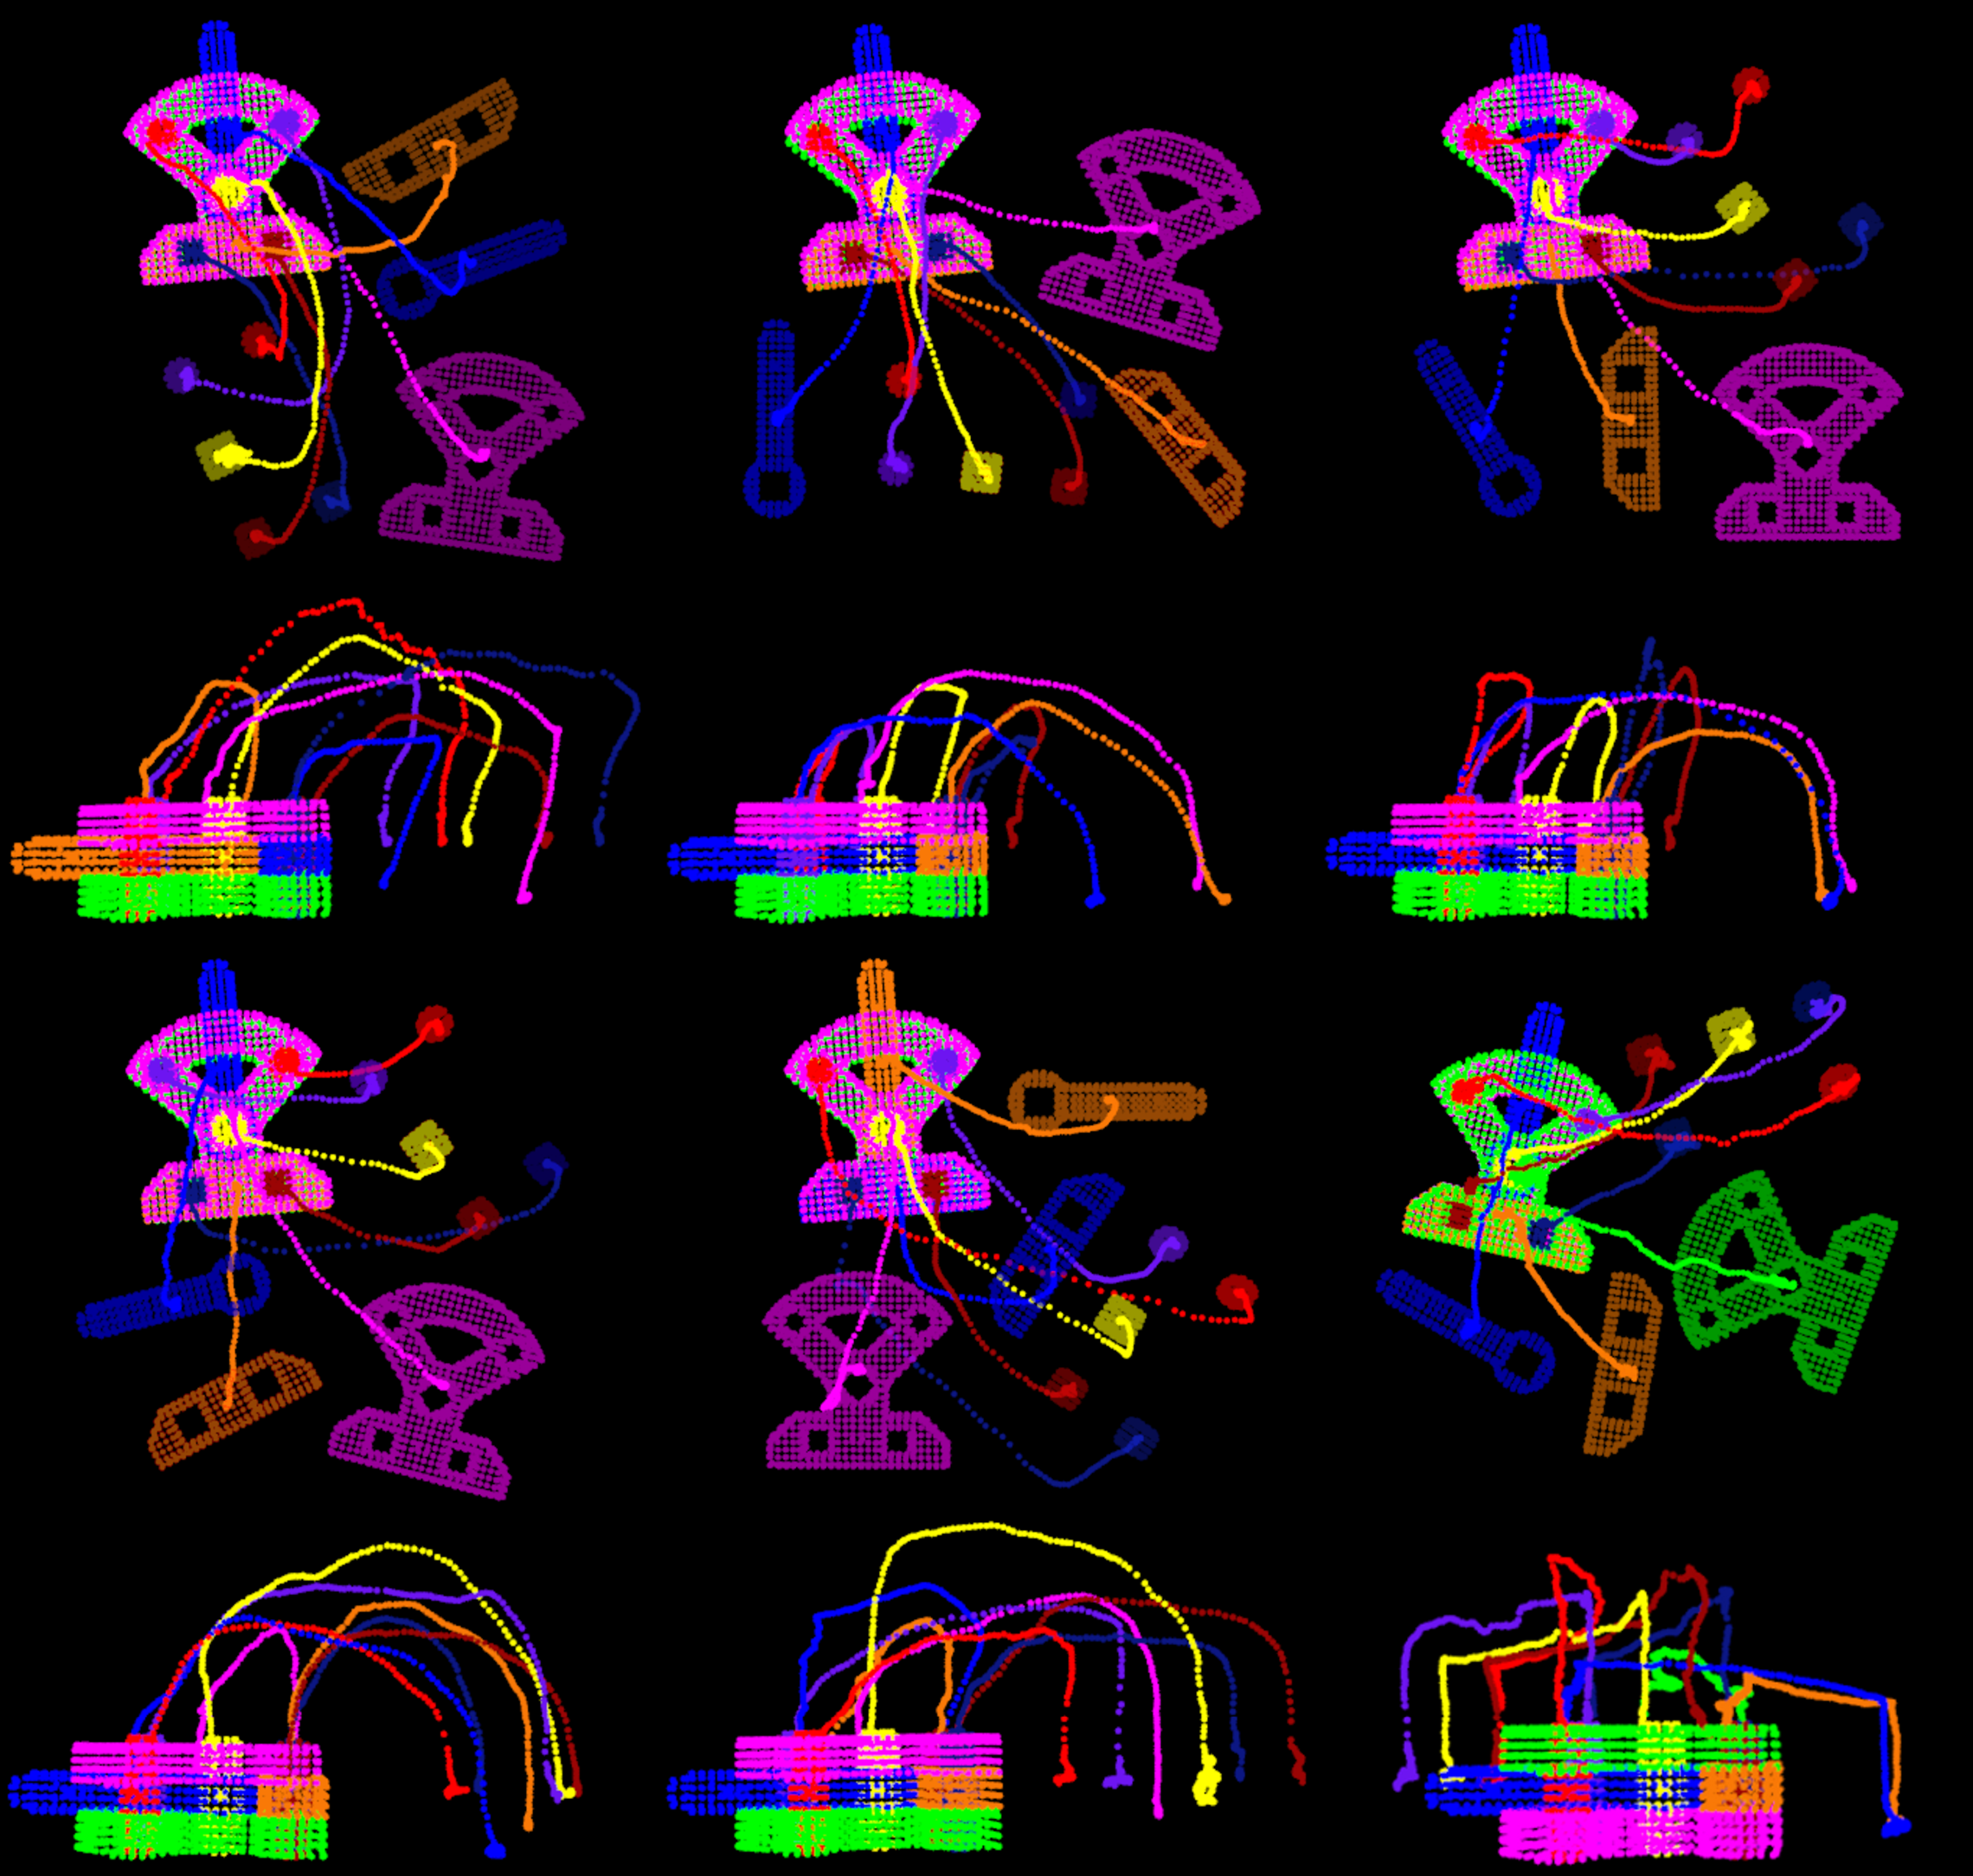
\includegraphics[width=1.0\textwidth]{figures/Tracking/TracksMontage.pdf}
  \caption[Snapshots from Virtual Reality Benchmark Run]{Tracking results from six different recordings of the Cranfield Scenario. The tracks in the bottom right corner are from the robot constructing the object, while the other five are from five different human demonstrators. In the overhead views, starting poses are shown (in slightly darker colors) for the objects.}
  \label{fig:TrackingResults}
\end{figure*}

\section{Discussion}
In this Chapter we have presented a novel spatially stratified sampling approach which greatly reduces the computational complexity of 3D Point Cloud correspondence particle filters. We evaluated the tracker using synthetic sequences for which precise ground truth exists, as well as real sequences of a human demonstration application. To demonstrate the effect of stratified sampling on performance, we conducted a sweep over the parameter space of number of particles and samples. This sweep showed the clear effectiveness of the proposed method in matching and even out-performing a GPU implementation on the CPU. 

We have now established our ability to track multiple objects in real-time within point cloud data. In the next Chapter, we will combine this tracker with the supervoxels presented previously to generate a full segmentation of point cloud video that is robust to occlusion and maintains object identities throughout extended sequences. To do this, we shall borrow some ideas from our 2D tracker presented in Chapter~\ref{Chap:VideoSegRelaxation}, and introduce a new global energy function that allows us to assign newly observed supervoxels to tracked targets.

